\documentclass[10pt,journal,compsoc]{IEEEtran}
\usepackage{tikz}
\usepackage{framed,graphicx}
\usepackage{multirow}
\usepackage{amsmath}
\usepackage{bigstrut}
\usepackage{color}
\usepackage{float}
\usepackage{graphics}
\usepackage{dblfloatfix}
\usepackage{colortbl}
\usepackage[scaled=1]{helvet} 
\usepackage{balance}
\usepackage[shortlabels]{enumitem}
\usepackage{url}
\usepackage[framed]{ntheorem}
\usepackage{framed}
\usepackage{hyperref}
% \usepackage{subcaption}
\usepackage{subfig}% http://ctan.org/pkg/subfig

%%% Color Definitions
\definecolor{lightgray}{gray}{0.8}
\definecolor{darkgray}{gray}{0.5}
\definecolor{lightgreen}{rgb}{.68, .79, .46}
\definecolor{lavenderpink}{gray}{0.92}
\definecolor{celadon}{gray}{0.7}
\definecolor{Gray}{gray}{0.9}
\definecolor{LightGray}{gray}{0.975}
\definecolor{cellgrey}{rgb}{.87, .87, .87}
\definecolor{steel}{rgb}{.11, .11, .7}
\definecolor{shadecolor}{gray}{0.95}

\newcommand{\result}[1]{
\vspace{0.2cm}
\noindent\begin{minipage}{\linewidth}
    \begin{tabular}{|p{0.95\linewidth}|}
    	\arrayrulecolor{Gray}
    	\hline\vspace{-0.2cm}
    	\rowcolor{Gray} \textit{\textbf{Result:}} #1\\\hline
    \end{tabular}
\end{minipage}\bigstrut%\\[-.2cm]
}

%%% Dr. M's shorthands
\newcommand{\bi}{\begin{itemize}} %[leftmargin=0.4cm]}
\newcommand{\ei}{\end{itemize}}
\newcommand{\be}{\begin{enumerate}}
\newcommand{\ee}{\end{enumerate}}
\newcommand{\tion}[1]{\S\ref{sect:#1}}
\newcommand{\fig}[1]{Figure~\ref{fig:#1}}
\newcommand{\tab}[1]{Table ~\ref{tab:#1}}
\newcommand{\eq}[1]{Equation~\ref{eq:#1}}
\newcommand{\review}[1]{\noindent\textit{#1\\}}

\pagenumbering{arabic} 

\bstctlcite{IEEEexample:BSTcontrol}

\begin{document}
	
\author{Rahul Krishna, Tim Menzies\\
	Comptuer Science, North Carolina State University, USA\\
	\{i.m.ralk, tim.menzies\}\@gmail.com
}

\IEEEtitleabstractindextext{%
\begin{abstract}

The current generation of software analytics tools are mostly  prediction algorithms (e.g. support vector machines, naive bayes, logistic regression, etc). While prediction is useful, after prediction comes {\em planning} about what actions to take in order to  improve quality. This research seeks methods that support actionable  analytics  that  offer  clear  guidance  on  ``what  to  do'' within the context of  a specific software project. Specifically, we propose the BELLTREE algorithm for generating   plans to improve software quality. Each such plan has the property that, if followed, it reduces the probability of future defect reports. When compared to other planning algorithms from the SE literature, we find that BELLTREE is most effective at learning plans from one project, then applying those plans to another. 

\end{abstract}

\noindent

\begin{IEEEkeywords}
      Data mining, actionable analytics, planning, bellwethers, local models, defect prediction.
\end{IEEEkeywords}}

\IEEEdisplaynontitleabstractindextext
    
\title{Planning Effective Changes Within and Across Software Projects}

\maketitle

\section{Introduction}

	Data mining tools have been applied to many applications in SE. For example, it has been used to  estimate	how long it would take to integrate new code into an existing project~\cite{czer11},	where bugs are most likely to occur~\cite{ostrand04,Menzies2007a}, or how long	it will take to develop this code~\cite{turhan11,koc11b}, etc.  Large organizations like Microsoft routinely practice  data-driven policy development where	organizational policies are learned from an extensive analysis of large datasets~\cite{export:208800,theisen15}. 
	
	Despite these successes, there exists  some drawbacks with current
	software analytic tools. At a recent workshop on ``Actionable Analytics'' at the 2015 IEEE conference on
	Automated Software Engineering,
	business users were very vocal in their complaints about analytics~\cite{hihn15}.
	``Those tools tell us \textit{what is},'' said one business user, ``But they don't tell us \textit{what to do}''.
	
	Accordingly, in this research, we seek new tools that support actionable analytics that offer  clear guidance on ``what to do'' about a specific software project. We seek new tools since the current generation of software analytics tools are mostly \textit{prediction} algorithms such as support vector machines~\cite{cortes95}, naive Bayes classifiers~\cite{lessmann08}, logistic regression~\cite{lessmann08}, etc. For example, defect prediction tools report what combinations of software project features predict for some dependent variable (such as the number of defects). Note that this is a different task to \textit{planning}, which answers the question: what to {\em change} in order to {\em improve} quality.
		
	More specifically, we seek  plans that offer {\em least} changes in software but most \textit{improve} the \textit{quality} where:
	\bi
	\item \textit{Quality} = defects reported by the development team; 
	\item \textit{Improvement} = lowered likelihood of future defects.
	\ei

	This paper advocates the use of the {\em bellwether effect}~\cite{krishna16} to generate plans. This effect states that:
    \begin{quote}
        \textit{`` \ldots When a community of programmers work on a set of projects, then within that community there exists one exemplary project, called the bellwether\footnote{According to the Oxford English Dictionary, the bellwether is the leading sheep of a flock, with a bell on its neck.}, which can best define quality predictors for the other projects \ldots ''}
    \end{quote}
   
    Utilizing  the bellwether effect, we propose a variant of our XTREE contrast set learner~\cite{krishna17a}  called ``BELLTREE''.  
    BELLTREE   searches for an exemplar project to construct plans for the other projects. These plans are then applied to all future data generated by that community. Bellwethers and BELLTREE are useful for planning purposes since:
    
    \bi
        \item These bellwethers are stable sources for planning. i.e., as long
        as the predictions of bellwethers remain the same, the lessons
        learned from it can be applied to the rest of the community.  
        \item As shown by the experiments of this this paper, bellwethers  can be found very early in a project’s life cycle (after
        analyzing only a few dozen code modules);
        \item Additionally, when compared to other planning methods in software engineering literature (Shatnawi~\cite{shatnawi}, Alves et al.~\cite{alves} and Oliveira et al.~\cite{oliveira}), BELLTREE produces much better plans.
    \ei

In summary, the contributions of this work are as follows.

\textit{1. New kinds of software analytics techniques:} This work combines planning~\cite{krishna17a} with cross-project learning using bellwethers~\cite{krishna16}. This is a unique approach since our previous work on bellwethers~\cite{krishna16, krishna17b} explored prediction and not planning as described here. Also, the previous work on planning~\cite{krishna17a} explored with-project problems but not cross-project problems as explored here. 

\textit{2. Compelling results about planning:} Our results show   that planning is quite successful in producing actions that can reduce the number of defects; e.g. our result show that our planners can reduce defects by more than 50\% in 6 out of the 8 datasets studied here ($>$90\% in the certain cases).

\textit{3. More evidence of generality of bellwethers:} The more the bellwether effect is explored, the more we learn about its broad
applicability. Originally, we explored this just in the context of prediction~\cite{krishna16},
it has been shown to work for defect prediction, effort estimation, predicting when issues will close, and detecting code smells~\cite{krishna17b}. This paper extends those results with a new finding that bellwethers can also be used from cross-project quality planning. This is an important result of much significance since, it suggests that general conclusions about SE are easily found (with bellwethers).

% \textit{4. Replication Package:} For readers this work who wish to replicate our findings, we have made available a replication package at https://git.io/v7c9k. 
 
%  The remainder of this section reviews our research questions along with a brief summary of our findings (see \tion{rqs}) and the connection of this work to our prior work in this area (see \tion{prior}).
%  After that, we answer some frequently asked questions questions about this work in \tion{faq}.  Following that, in \tion{background} we present some related work on planning in AI and in software engineering. \tion{prelim} revisits some of our previous findings in greater detail, there we (1) introduce the datasets used in this study, (2) discuss the verification oracles, and (3) introduce statistical validation tools used in this paper to assess the quality of these plans. In \tion{motivate}, we revisit the notion of planning and discuss how planning follows prediction. Specifically, we introduce the various planners that are studied in this report. We also discuss how these planners can be used to supplement decision making from a realistic standpoint. In \tion{results}, we offer answers to each of the research questions. We explore the treats to validity in \tion{threats}. Finally, we offer our conclusions and direction of future work in \tion{future}.

\subsection{Research Questions}
\label{sect:rqs}
% XTREE (and BELLTREE) are {\em Cluster + Contrast} \textit{planning} tools that work as follows:
% \bi
% \item \textit{Cluster} different parts of the software project based on a quality measure (e.g. the number of defects).
% \item  Report the \textit{contrast sets} between neighboring clusters.
% \ei 

% Each of these contrast sets represent the difference between these clusters and they can be interpreted as \textit{plans}. The rest of this section provides a brief overview of the research questions this paper seeks to answer.

This section provides a brief overview of the research questions this paper seeks to answer.

\subsection*{RQ1: How similar are the plans generated by XTREE with those undertaken by developers?}

In the first research question, we seek to establish the similarity between the 
plans generated by XTREE and the outcome of developers' changes to projects. If 
the plans offered by XTREE do not match those undertaken by developers, then it 
becomes difficult to justify the effectiveness of XTREE in generating 
actionable plans.\\[-0.1cm]

\noindent\begin{minipage}{\linewidth}
	\begin{tabular}{|p{0.95\linewidth}|}
		\arrayrulecolor{Gray}
		\hline\vspace{-0.2cm}
		\cellcolor{Gray}\textit{\textbf{Result:}} In all the projects studied here, 
		there is a significant overlap between plans recommended by XTREE and those 
		undertaken by developers.\\\hline
	\end{tabular}
\end{minipage}\bigstrut\\[-.4cm]


\subsection*{RQ2: How effective is within-project planning with XTREE?}

In this research question, we assess the effectiveness of XTREE when it is trained on past data from \textit{within} a project. This research question follows RQ1, where we showed that changes recommended by XTREE has a significant overlap with changes actually undertaken by developers. XTREE recommends changes so that the project might have have fewer defects in the next version, however correlation does not necessarily imply causation, it is theoretically possible that the recommendations generated by XTREE could be misleading. 

The  results of this paper are in accordance with our previous 
findings~\cite{krishna17a} and show that {\em XTREE} is an effective planner 
for automatically recommending useful plans.\\[-0.1cm]


\noindent\begin{minipage}{\linewidth}
	\begin{tabular}{|p{0.95\linewidth}|}
		\arrayrulecolor{Gray}
		\hline\vspace{-0.2cm}
		\cellcolor{Gray}\textit{\textbf{Result:}} For within-project planning, we see 
		that greater the overlap with XTREE's recommendations the larger the number 
		of defects reduced in a subsequent release of a project. This was true in 8 
		out of 9 projects studied here.\\\hline
	\end{tabular}
\end{minipage}\bigstrut\\[-.4cm]


     
\subsection*{RQ3: How does XTREE compare with other threshold based methods for within-project planning?}
    
Alternative methods for planning make use of statistically determined thresholds over source code metrics for reducing defects. Recent work by Shatnawi~\cite{shatnawi}, Alves et al.~\cite{alves}, and Oliveira et al.~\cite{oliveira} assume that unusually large measurements in source code metrics point to larger likelihood of defects and these should be avoided since, if left unchanged, they would lead to defect-prone code.  

Our results show  that their assumption is not effective to generate actionable 
plans  and that XTREE is a better way to plan quality improvement.\\[-0.1cm]

\noindent\begin{minipage}{\linewidth}
	\begin{tabular}{|p{0.95\linewidth}|}
		\arrayrulecolor{Gray}
		\hline\vspace{-0.2cm}
		\cellcolor{Gray}\textit{\textbf{Result:}} For within-project planning, plans 
		generated by XTREE is significantly superior to plans generated by other 
		threshold based methods.\\\hline
	\end{tabular}
\end{minipage}\bigstrut\\[-.4cm]


\subsection*{RQ4: How effective is cross-project planning with XTREE?}
    
When projects do not have sufficient within project data (perhaps due to the project being relatively new), we may use data from other similar projects to generate actionable plans for the original project. We achieve this using the \textit{bellwether effect}~\cite{krishna17a}. We first discover a \textit{bellwether} dataset from the available projects, and then we train XTREE on the bellwether data. In this research question, we assess the effectiveness of plans when using the \textit{bellwether} data.

As with RQ2, we see that in a cross-project setting, plans generated using 
XTREE and the bellwether data is quite effective in generating actionable 
plans.\\[-.4cm]


\noindent\begin{minipage}{\linewidth}
	\begin{tabular}{|p{0.95\linewidth}|}
		\arrayrulecolor{Gray}
		\hline\vspace{-0.2cm}
		\cellcolor{Gray}\textit{\textbf{Result:}} For cross-project planning, we see 
		that larger the overlap with XTREE's recommendations leads to larger 
		reduction in the number of defects for subsequent release of a project. This 
		was true in all 9 projects that were studied here.\\\hline
	\end{tabular}
\end{minipage}\bigstrut\\[-.4cm]

\subsection*{RQ5: Are cross-project plans generated by XTREE comparable to within-project plans?}

In RQ4, we established that it is possible to generate effective plans for projects by a training a planner (XTREE) on a \textit{bellwether} data. In this research question, we compare plans generated using within-project data to those generated using cross-project data (the bellwether dataset).

Our experiments show that the effectiveness of plans generated from within-project data and XTREE is statistically comparable to plans derived cross-project data using the bellwether dataset. And since the source of data used for cross-project planning is the bellwether, it remains unchanged for relative longer stretches to time~\cite{krishna17a}. This means that the plans would also remain consistent for long stretches of time. This result is particularly encouraging since it demonstrates a level of conclusion stability required to maintain user confidence in analytics.

\noindent\begin{minipage}{\linewidth}
	\begin{tabular}{|p{0.95\linewidth}|}
		\arrayrulecolor{Gray}
		\hline\vspace{-0.2cm}
		\cellcolor{Gray}\textit{\textbf{Result:}} Cross-project planning with XTREE 
		is statistically comparable to within-project planning.\\\hline
	\end{tabular}
\end{minipage}\bigstrut%\\[-.2cm]

    
\subsection*{RQ6: Are  BELLTREE  cross-project  plans  any  better  than XTREE’s within project plans?}
    
In the final research question, we compare plans of XTREE and alternative threshold based methods of Shatnawi~\cite{shatnawi}, Alves et al.~\cite{alves}, and Oliveira et al.~\cite{oliveira} for cross-project planning with the bellwether data.

As with RQ4, our results show that threshold based methods not effective in generating actionable plans for cross-project planning. XTREE is a significantly superior approach to cross-project planning.

\noindent\begin{minipage}{\linewidth}
	\begin{tabular}{|p{0.95\linewidth}|}
		\arrayrulecolor{Gray}
		\hline\vspace{-0.2cm}
		\cellcolor{Gray}\textit{\textbf{Result:}} For cross-project planning, plans 
		generated by XTREE is significantly better 
		than to plans generated by other threshold based methods.\\\hline
	\end{tabular}
\end{minipage}\bigstrut%\\[-.2cm]


\section{Motivation}
\label{sect:motivate}

\begin{figure}[!t]
    \centering
    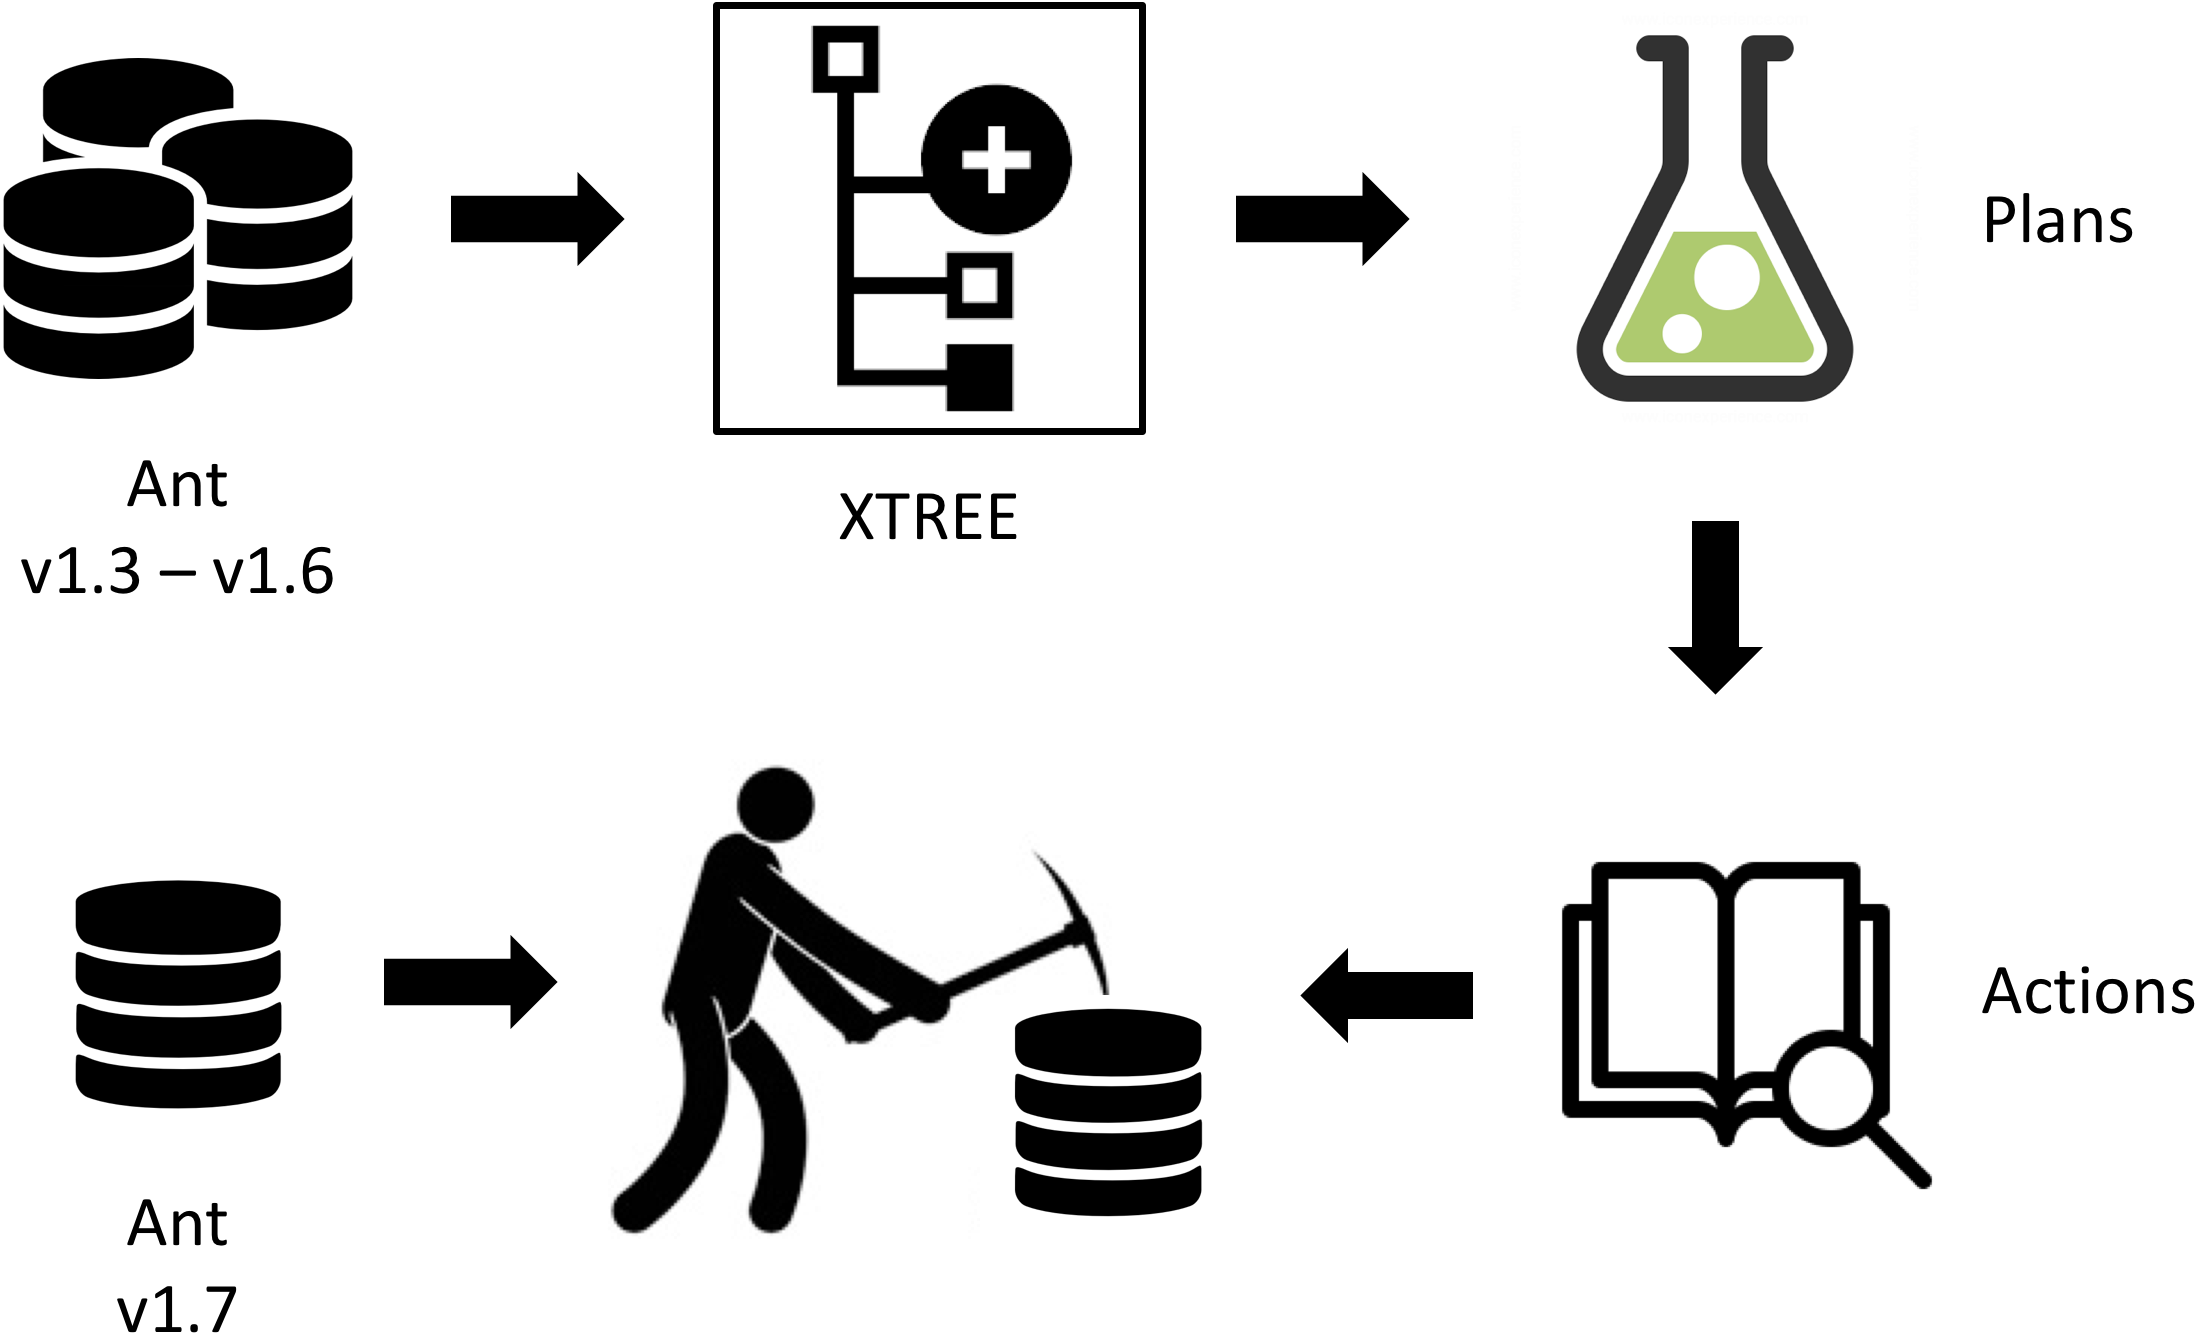
\includegraphics[width=\linewidth]{images/example.png}
    \caption{A proposed planning framework.}
    \label{fig:flowchart}
\end{figure}

\begin{figure}
\centering
\captionsetup[subfigure]{width=\linewidth}
\subfloat[subfig:plans][Plans recommended by XTREE]{
\resizebox{0.8\linewidth}{!}{
\begin{tabular}{ccccccccc}
\hline
\rowcolor{Gray} DIT & NOC & CBO & RFC & FOUT & WMC & NOM & LOC & LCOM \\
$\cdot$ & $\cdot$    & $\cdot$    & $+$   & $\cdot$     & $+$   & $+$   & $+$   
& $+$    \\\hline
\end{tabular}}
\label{subfig:plans}
}\\

\subfloat[][A sample of possible actions developers can take. The action highlighted in \colorbox{lightgreen}{green} indicates the action that matches the recommendation offered by XTREE with respect the available metrics.]{
\resizebox{\linewidth}{!}{
\begin{tabular}{lccccccccc}
\hline
\rowcolor{Gray}Action                                      & DIT & NOC & CBO & RFC & FOUT & WMC & NOM & LOC & LCOM \\ 
Extract Class                               &     &     & $+$   & $-$   & $+$    & $-$   & $-$   & $-$   & $-$    \\
\rowcolor{lightgreen} Extract Method                              &     &     &     & $+$   &      & $+$   & $+$   & $+$   & $+$    \\
Hide Method                                 &     &     &     &     &      &     &     &     &      \\
Inline Method                               &     &     &     & $-$   &      & $-$   & $-$   & $-$   & $-$    \\
Inline Temp                                 &     &     &     &     &      &     &     & $-$   &      \\
Remove Setting Method                       &     &     &     & $-$   &      & $-$   & $-$   & $-$   & $-$    \\
Replace Assignment                          &     &     &     &     &      &     &     & $-$   &      \\
Replace Magic Number                        &     &     &     &     &      &     &     & $+$   &      \\
Consolidate Conditional                     &     &     &     & $+$   &      & $+$   & $+$   & $-$   & $+$    \\
Reverse Conditional                         &     &     &     &     &      &     &     &     &      \\
Encapsulate Field                           &     &     &     &     &      & $+$   & $+$   & $+$   & $+$    \\
Inline Class                                &     &     & $-$   & $+$   & $-$    & $+$   & $+$   & $+$   & $+$    \\ \hline
\end{tabular}}
\label{subfig:actions}
}

\subfloat[][A contrived example of a inventory management task which is possibly defective.]{
\fbox{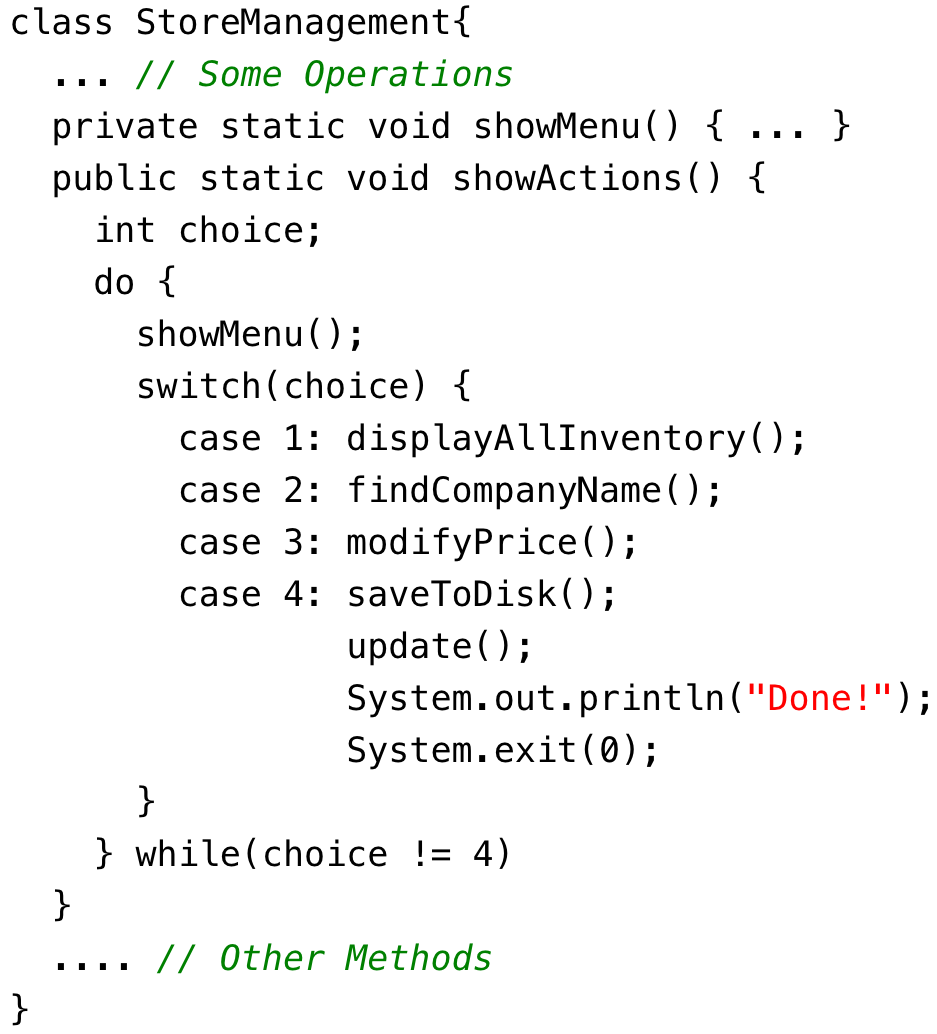
\includegraphics[width=0.64\linewidth]{images/before.png}}
\label{subfig:before}
}\\
\subfloat[subfig:after][The example in \ref{fig:motivating_example}\protect\subref{subfig:before} after applying ``extract method'' operation as per XTREE's recommendations.]{
\fbox{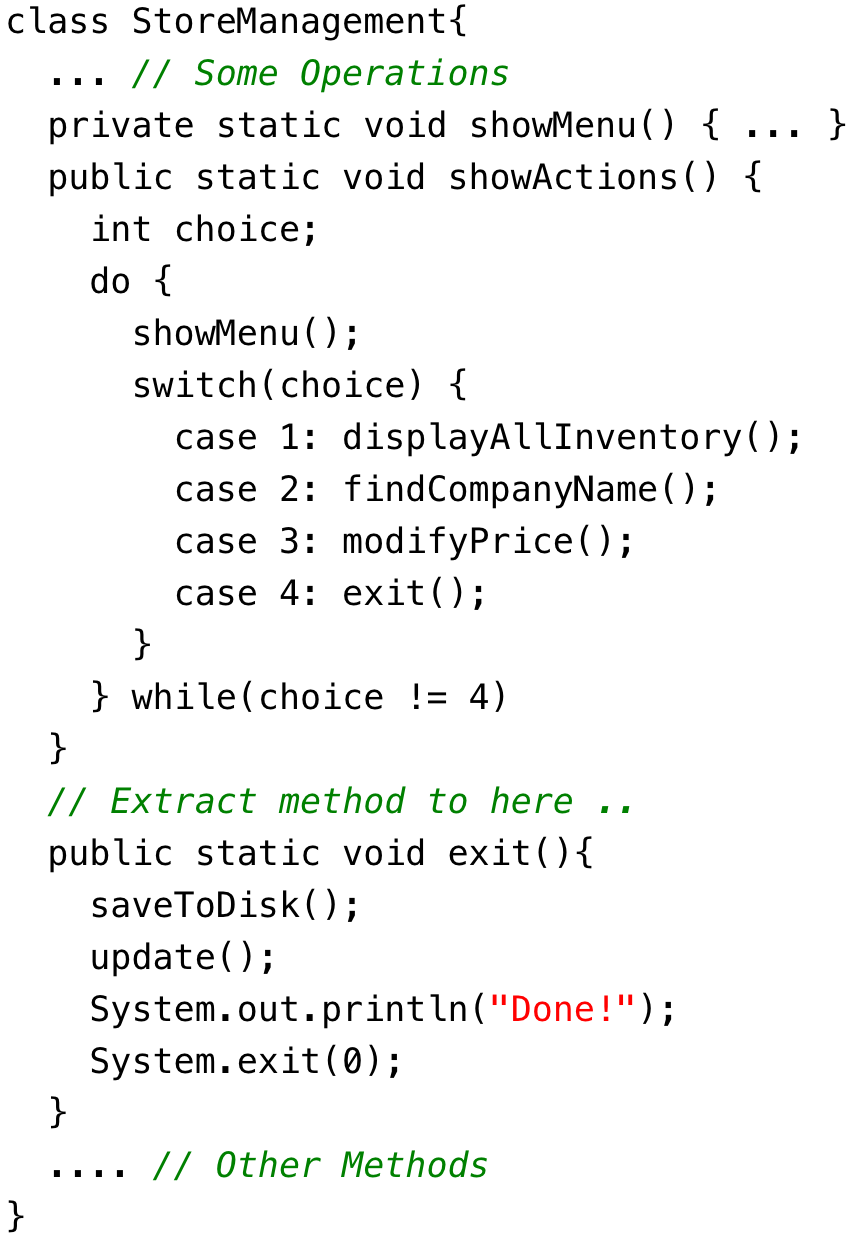
\includegraphics[width=0.64\linewidth]{images/after.png}}
\label{subfig:after}
}

\caption{An example of how developers might use XTREE to reduce software defects.}
\label{fig:motivating_example}
\end{figure}

\subsection{What exactly is ``planning"?}

We distinguish planning from prediction for software quality as follows: 
Quality prediction points to the likelihood of defects. Predictors take the form:
\begin{equation*}
    out = f(in)    
\end{equation*}
where {\em in} contains many independent features (such as OO metrics) and {\em out} contains some measure of
how many defects are present. For software analytics, the function $f$ is learned via data mining (for static code attributes for instance).

On the other hand, quality planning generates a concrete set of actions that can be taken (as precautionary measures) to significantly reduce the likelihood of defects occurring in the future.

For a formal definition of plans, consider a defective test example $Z$, a planner
proposes a plan $D$ to adjust attribute $Z_j$ as follows:

{\small\[
\forall \delta_j \in \Delta :  Z_j =  
\begin{cases}
     Z_j + \delta_j& \text{if $Z_j$ is numeric}\\
    \delta_j              & \text{otherwise}
\end{cases}
\]}

With this planner, to (say) simplify a large bug-prone method, our planners
might suggest to a developer to reduce its size (i.e. refactor that
code by, say, splitting it across two simpler functions).

\subsection{Example}


The proposed framework for the use of XTREE in a real world situation is illustrated in \fig{flowchart}. There we see that given within-project data\footnote{This within-project data can easily be replaced by the bellwether dataset if necessary.} in the form of data from previous releases of a sample project (releases v1.3 --- v1.6), we first construct a planner (XTREE). Then using the test data (Ant v1.7), we obtain plans for what changes can be made to improve the quality of the software. Next, we look for specific actions that can be taken (for some example actions, see \fig{motivating_example}\protect\subref{subfig:actions}). When a plan recommended by XTREE matches possible action, the developers may choose to use the plan as a guide to undertaking preventive or perfective  actions to improve the quality of that software.


For a more concrete example, consider \fig{motivating_example}. Here, we apply the framework proposed in \fig{flowchart} and obtain a set of recommendations as shown in \ref{fig:motivating_example}\protect\subref{subfig:plans}. Then, we use \ref{fig:motivating_example}\protect\subref{subfig:actions} to look-up possible actions developers may take, there we see that performing an ``extract method'' operation may help alleviate certain defects (this is highlighted in {\colorbox{lightgreen}{green}}). 

In \ref{fig:motivating_example}\protect\subref{subfig:before} we show a simple contrived example of a class where the above operation may be performed. In \ref{fig:motivating_example}\protect\subref{subfig:after}, we demostrate how a developer may go about performing the ``extract method'' operation.

\subsection{Planning in Classical AI}

In classical AI, planning usually refers to generating a sequence of actions that enables an \textit{agent} to achieve a specific \textit{goal}~\cite{norvig}. In an idealized situation, it is assumed that the possible initial states of the world is known and so are the description of the desired goal in addition to the set of possible and feasible actions. In such a hypothetical situation, planning results in generating a set of actions that is guaranteed to enable one to reach a desired goal. This can be achieved by classical search-based problem solving  approaches or logical planning agents. Such planning tasks now play a significant role in a variety of demanding applications, ranging from controlling space vehicles and robots to playing the game of bridge~\cite{ghallab04}. 

As discussed in the rest this section, there are many  types of planning. We introduce the premise of those different planning paradigms, then dedicate the rest of the section to discuss its implications for planning in software engineering.

\subsubsection{Classical Planning}
A simple abstraction of the planning problem is known as classical planning. Classical planning assumes that the initial state is fully-observable and any action is deterministic. Such an assumption enables us to predict the outcome of an action accurately every single time. Further, plans can be defined as sequences of actions, because it is always known in advance which actions will be needed~\cite{strips}. 

Classical Planning is most useful when the problem is not very complex and the simplifying assumptions mentioned above lead to a development of a well-founded model~\cite{wooldridge95}.  In the case of complex domains like software engineering, performing a search of plans is highly inefficient. It becomes very difficult to pick the correct search space, algorithm, and heuristics for finding these plans~\cite{ghallab04}.

\subsubsection{Probabilistic Planning}
\label{sect:prob_plan}
Probabilistic planning tackles a slightly different problem in planning --- one where the outcomes may be random and are partly controlled by the decision maker~\cite{Bel, altman99, guo2009}. These kinds of planning problems are usually solved using dynamic programming and reinforcement learning. The key idea here is to represent the planning problem as an optimization problem~\cite{ghallab04}. Planning for such problems are best achieved when the state-space is small~\cite{ghallab04}. Additionally, such a planning approach works even with partial observability, i.e., it works even when the planning agent cannot fully observe the underlying problem space. Planning over partially observable states is achieved by maintaining a distribution of probabilities over the possible states and planning based on these distributions~\cite{kaelbling98}.


\subsubsection{Preference-based Planning}
\label{sect:pref_plan}
The preference based planning is an extension of the above planning schemes with a focus on producing plans that satisfy as many user-defined constraints (preferences) as possible~\cite{son06}. These preferences as defined by the user are generally not hard constrains, rather they define the quality of the plan, which increases as more of the preferences are satisfied. Algorithms that can solve constraint satisfaction problems are well suited to solve these forms of planning problems. Other popular algorithms include PPLAN~\cite{son06} and HTN~\cite{baier09}. However, existence of a model precludes the use of this planning approach. This is a major impediment, since for reasons discussed in the following section, not every domain has a reliable model.

\subsection{Planning in Software Engineering}
We know of at least two kinds of planning research in SE. Each kind is distinguishable by {\em what} is being changed.

In {\em test-based planning}, some optimization is applied to reduce the number of tests required to achieve to a certain goal  or the time taken before tests yield interesting results~\cite{tallam2006concept, yoo2012regression, blue2013interaction}.
% \begin{figure*}[!t]
% 	\arrayrulecolor{lightgray}
% 	\centering
% 	\resizebox{\linewidth}{!}{%
% 		\begin{tabular}{r|l|l}
% 			wmc & weighted methods per class & \\\hline
% 			dit & depth of inheritance tree & \\\hline
% 			noc &  number of children & \\\hline
% 			cbo & coupling between objects & increased when the methods of one
% 			class access services of another. \\\hline
% 			rfc & response for a class &number of  methods invoked in response to
% 			a message to the object. \\\hline
% 			lcom & lack of cohesion in methods &number of pairs of methods that do
% 			not share a reference to an instance variable. \\\hline
% 			ca & afferent couplings & how many other classes use the specific
% 			class.  \\\hline
% 			ce & efferent couplings & how many other classes is used by the
% 			specific class.  \\\hline
% 			npm & number of public methods &  \\\hline
% 			locm3 & another lack of cohesion measure & if $m,a$ are  the number of
% 			$methods,attributes$
% 			in a class number and $\mu(a)$  is the number of methods accessing an
% 			attribute, 
% 			then
% 			$lcom3=((\frac{1}{a} \sum_j^a \mu(a_j)) - m)/ (1-m)$.
% 			\\\hline
% 			loc & lines of code & \\\hline
% 			dam & data access & ratio of  private (protected)
% 			attributes to   total   attributes \\\hline
% 			moa &  aggregation &  count of the number of data declarations (class
% 			fields) whose types are user defined classes \\\hline
% 			mfa & functional abstraction & number of methods inherited by a class
% 			plus number of methods accessible by member methods of the
% 			class \\\hline
% 			cam & cohesion amongst classes & summation of number of different
% 			types of method parameters in every method divided by a multiplication
% 			of number of different method parameter types in whole class and
% 			number of methods.  \\\hline
% 			ic & inheritance coupling &  number of parent classes to which a given
% 			class is coupled (includes counts of methods and variables inherited)
% 			\\\hline
% 			cbm &coupling between methods &  total number of new/redefined methods
% 			to which all the inherited methods are coupled \\\hline
% 			amc & average method complexity & e.g. number of JAVA byte codes \\\hline
% 			max\_cc & maximum McCabe & maximum McCabe's cyclomatic complexity seen
% 			in class \\\hline
% 			avg\_cc & average McCabe & average McCabe's cyclomatic complexity seen
% 			in class \\\hline
% 			\rowcolor{lightgray}
% 			defect & defect & Boolean: where defects found in post-release bug-tracking systems.
% 		\end{tabular}
% 	} 
% 	\caption{Sample static code attributes.}\label{fig:static_metrics}
% \end{figure*}

\begin{figure}
	\renewcommand{\baselinestretch}{0.7}\begin{center}
		\resizebox{0.8\linewidth}{!}{
			\begin{tabular}{c|l}
				amc & average method complexity \\\hline
				avg\, cc & average McCabe \\\hline
				ca & afferent couplings \\\hline
				cam & cohesion amongst classes \\\hline
				cbm & coupling between methods \\\hline
				cbo & coupling between objects \\\hline
				ce & efferent couplings \\\hline
				dam & data access\\\hline
				dit & depth of inheritance tree\\\hline
				ic & inheritance coupling\\\hline
				lcom (lcom3) & 2 measures of lack of cohesion in methods \\\hline
				loc & lines of code \\\hline
				max\, cc & maximum McCabe\\\hline
				mfa & functional abstraction\\\hline
				moa &  aggregation\\\hline
				noc &  number of children\\\hline
				npm & number of public methods\\\hline
				rfc & response for a class\\\hline
				wmc & weighted methods per class\\\hline
				\rowcolor{lightgray}
				\#defects & raw defect counts\\
			\end{tabular}
		}
	\end{center}
	\caption{OO code metrics used for all studies in this paper.
	   Last line, shown in \colorbox{lightgray}{gray}, denotes the dependent variable. For more details, see~\cite{krishna17a}.}\label{fig:static_metrics}
\end{figure}


In {\em process-based planning} some search-based optimizer is applied to a software process model to infer high-level business plans about software projects. Examples of that kind of work include our own prior studies combining simulated annealing with the COCOMO models or Ruhe et al.'s work on next release planning in requirements engineering~\cite{ruhe2003quantitative, ruhe2010product}. This paper is about {\em code-based planning} where the goal is to change a code base in order to improve that code in some way.

In software engineering, the planning problem translates to proposing changes to software artifacts. These are usually a hybrid task combining elements of probabilistic planning (see \tion{prob_plan}) and preference based plans (see \tion{pref_plan}). Solving this has been undertaken via the use of some search-based software engineering techniques~\cite{Harman2009, Harman2011}. These search-based techniques are evolutionary algorithms that propose actions guided by a fitness function derived from a well established domain model. They work by: (a) generating an initial population of solutions using an initialization policy (for example they may generate 100s to 100000s instances via random sampling); (b) evaluating each solution using a problem specific fitness function, (c) creating new solutions via mutation and crossover operation of existing samples, and (d) reassessing these solutions using the fitness functions. Examples of algorithms include GALE, NSGA-II, NSGA-III, SPEA2, IBEA, MOEA/D, etc.~\cite{krall2015gale,deb00a,zit02,zit04, deb14,Cui2005a,zhang07:TEC}. 
\begin{figure}[!t]

\centering
\begin{minipage}{\linewidth}
\resizebox{\linewidth}{!}{%
% Table generated by Excel2LaTeX from sheet 'Sheet1'
\scriptsize \begin{tabular}{l|r|r|r}
\hline
\cline{2-4}  Dataset     & \multicolumn{1}{r|}{Versions} & \multicolumn{1}{l|}{\# samples} & Bugs (\%) \bigstrut\\
\hline
 \cellcolor{lavenderpink}Lucene & \multicolumn{1}{r
|}{\cellcolor{lavenderpink}2.0, 2.2,2.4} & \cellcolor{lavenderpink}782   & \cellcolor{lavenderpink}438 (56.01) \\
 Ant   & \multicolumn{1}{r|}{1.3, 1.4, 1.5, 1.6, 1.7} & 1692  & 350 (20.69) \\
 Ivy   & \multicolumn{1}{r|}{1.1, 1.4,2.0} & 704   & 119 (16.90) \\
 Jedit & \multicolumn{1}{r|}{3.2, 4.0, 4.1, 4.2,4.3} & 1749  & 303 (17.32) \\
 Poi   & \multicolumn{1}{r|}{1.5, 2, 2.5, 3.0} & 1378  & 707 (51.31) \\
       Camel & \multicolumn{1}{r|}{1.0, 1.2, 1.4,1.6} & 2784  & 562 (20.19) \\
       Log4j & \multicolumn{1}{r|}{1.0, 1.1,1.2} & 449   & 260 (57.91) \\
       Velocity & \multicolumn{1}{r|}{1.4, 1.5,1.6} & 639   & 367 (57.43) \\
       Xalan & \multicolumn{1}{r|}{2.4, 2.5, 2.6,2.7} & 3320  & 1806 (54.40) \\
       Xerces & \multicolumn{1}{r|}{1.0, 1.2, 1.3,1.4} & 1643  & 654 (39.81) \\
\hline
% \multirow{5}[2]{*}{AEEEM} & \cellcolor{lavenderpink}LC    &    \cellcolor{lavenderpink}   & \cellcolor{lavenderpink}399   & \cellcolor{lavenderpink}64 (9.26) \\
% & JDT   &       & 997   & 206 (20.66) \\
% & ML    &       & 1826  & 245 (13.16) \\
% & PDE   &       & 1492  & 209 (13.96) \\
%       & EQ    &       & 325   & 129 (39.81) \\
% \hline
% \multirow{3}[2]{*}{ReLink} & \cellcolor{lavenderpink}Safe  &   \cellcolor{lavenderpink}    & \cellcolor{lavenderpink}56    & \cellcolor{lavenderpink}22 (39.29) \\
% & Apache &       & 194   & 98 (50.52) \\
%       & Zxing &       & 399   & 118 (29.57) \\
% \hline
\end{tabular}%
}
% \end{minipage}~\begin{minipage}{.36\linewidth}
% \resizebox{\linewidth}{!}{%
% % Table generated by Excel2LaTeX from sheet 'Sheet1'
% \begin{tabular}{|rrrr|c|c}
% \hline
% \multicolumn{4}{|c|}{\multirow{2}[4]{*}{Description}}& \multirow{2}[4]{*}{\# metrics} & \multirow{2}[4]{*}{Granularity} \bigstrut\\
% % & &  &       &  \bigstrut\\
%       &       &       &       & \multirow{10}[4]{*}{20} & \multirow{10}[4]{*}{Class} \\\hline
%       &       &       &       & &  \\
%       &       &       &       & & \\
%       &       &       &       & & \\
%       &       &       &       & & \\
%       &       &       &       & & \\
%       &       &       &       & & \\
%       &       &       &       & & \\
%       &       &       &       & & \\
%       &       &       &       & & \\\hline
% %       &       &       &       & \multirow{5}[2]{*}{61} & \multirow{5}[2]{*}{class} \\
% % 63    & 9     & 18    & 4     &       &  \\
% % 67    & 11    & 24    & 14    &       &  \\
% % 61    & 6     & 13    & 2     &       &  \\
% % 27    & 8     & 6     & 8     &       &  \\
% % \hline
% %       &       &       &       & \multirow{3}[2]{*}{26} & \multirow{3}[2]{*}{file} \\
% % 85    & 4     & 38    & 14    &       &  \\
% % 28    & 29    & 14    & 10    &       &  \\
% % \hline
% \end{tabular}%
% }
\end{minipage}
\caption{The figure lists defect datasets used in this paper. The bellwether dataset is highlighted in \colorbox{lavenderpink}{light gray}.}
\label{fig:datasets}
\end{figure} 
These planning tools all require access to some trustworthy models that can be used to explore some highly novel examples. In some software engineering domains there is ready access to such models which can offer assessment of newly generated plans. Examples of such domains within software engineering include automated program repair~\cite{Weimer2009, Forrest2009, Goues12, Schulte2010, LeGoues2015}, software product line management~\cite{clements2002software, sayyad13, metzger14, henard15}, automated test generation~\cite{me09m,andrews07,andrews10}, etc.  

However, not all domains come with ready-to-use models. For example, consider software defect prediction and all the intricate issues that may lead to defects in a product. A model that includes {\em all} those potential issues would be very large and complex. Further, the empirical data required to validate any/all parts of that model can be hard to find.


In fact, our experience has been that accessing and/or commissioning a model can be a labor-intensive process.
For  example, in previous work~\cite{me07f} we used models developed by Boehm's group at the University of Southern California.
Those models inputted project descriptors to output predictors of development effort, project risk, and defects.
Some of those models took decades to develop and mature (from 1981~\cite{boehm81} to 2000~\cite{boehm00b}). 

Furthermore, even when there is an existing model, they can require constant  maintenance lest they become out-dated. Elsewhere, we have described our extensions to the USC models to enable reasoning about agile software developments. It took many months to implement and certify those extensions~\cite{me09i,me09j}. The problem of model maintenance is another motivation to look for alternate methods that can be automatically updated with new data.

Fortunately, sometimes  it is easier to access cases of a model's behaviour than the model itself. For example, in prior work with Martin  Feather from the Jet Propulsion Laboratory~\cite{fea02a},  our research partner could not share a propriety model from within the NASA firewalls. However, they could share logs of the input/output of that model.

In summary, for domains with readily accessible models, we recommend
the kinds of tools that are widely used in the search-based
software engineering community such as GALE, NSGA-II, NSGA-III, SPEA2, IBEA, particle swarm optimization, MOEA/D, etc. In several other cases where this is not an option, we propose the use of data mining approaches to create a quasi-model of the domain 
and make of use observable states from this data to generate an estimation of the model. Our preferred tools in this paper XTREE and BELLTREE take this approach and as presented elsewhere in this paper, these methodologies have very encouraging results.


\section{Research Methods}
\label{sect:prelim}
\subsection{Datasets}
\label{sect:data}
The defect dataset used in this study comprises a total of 49 datasets grouped into 3 communities taken
from previous transfer learning studies. The projects measure defects at various levels of granularity ranging from class-level to file-level. All the datasets are described in the attributes of \fig{static_metrics}.
\fig{datasets} summarizes all the communities of datasets used in our experiments. 

Since we attempt to transfer plans from within the project, we explore homogeneous
transfer of plans using the attributes shared by a community. We explored another community of dataset from the SEACRAFT repository\footnote{$\text{https://zenodo.org/communities/seacraft/}$}. Thisgroup of data contains defect measures from several Apache projects. 
It was gathered by Jureczko et al. \cite{Jureczko2010}. This dataset 
contains records the number of known defects for each class using a 
post-release bug tracking system. The classes are described in terms of 20 
OO metrics, including CK metrics and McCabes complexity metrics. Each 
dataset in the Apache community has several versions totalling 38 
different datasets. For more information on this dataset
see~\cite{krishna16}. 

\subsection{A Strategy for Evaluating Planners}
\begin{figure}[!t]
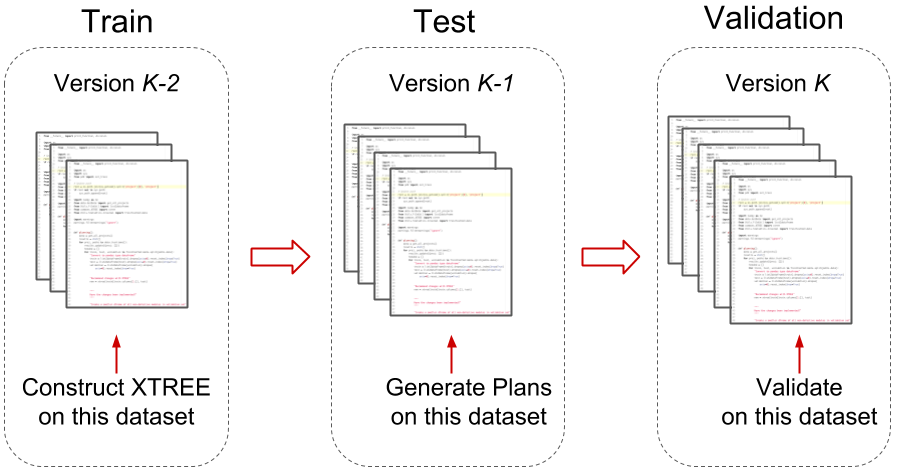
\includegraphics[width=\linewidth]{images/k_test.png}
\caption{K-Test to validate plans.}\label{fig:design}
\end{figure}

% \begin{figure}[!t]
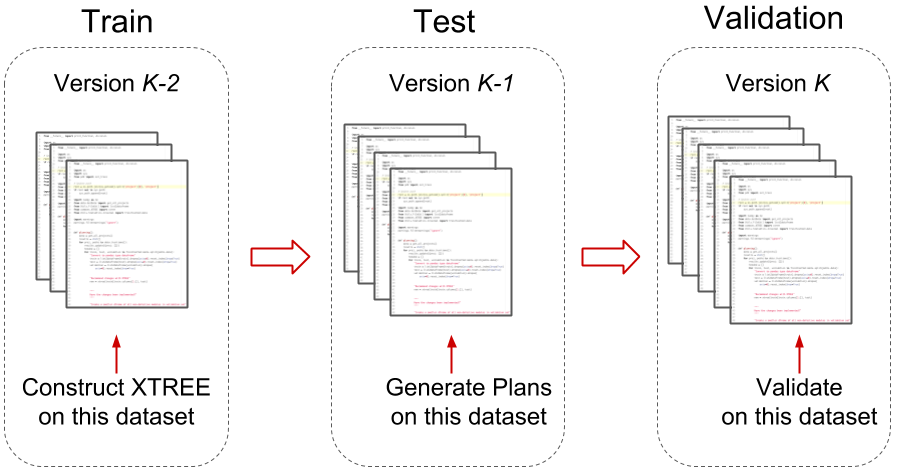
\includegraphics[width=\linewidth]{images/k_test.png}
\caption{K-Test to validate plans.}\label{fig:design}
\end{figure}

In \tion{planners} we describe the planners and a way to translate these plans into actionable decisions. To assess the effect of acting on these plans, we propose a  \textit{verification oracle}. This is necessary because it can be rather difficult  to judge the  effects of applying the plan. They cannot be assessed just by a rerun of the test suite for three reasons: (1) The defects were recorded by a post release bug tracking system. It is entirely possible it escaped detection by the existing test suite; (2) Rewriting test cases to enable coverage of all possible scenarios presents a significant challenge; and (3) It make take a significant amount of effort to write new test cases that identify these changes as they are made.

To resolve this problem, SE researchers such as
Cheng et al.~\cite{Cheng10}, O'Keefe et al.~\cite{OKeeffe08,OKeeffe07},
Moghadam~\cite{Moghadam2011} and Mkaouer et al.~\cite{Mkaouer14}
use a {\em verification oracle} that is learned separately from the primary oracle. The verification oracles assesses how defective the code is before and after some code changes. For their verification oracle, Cheng, O'Keefe, Moghadam and  Mkaouer et al. use the QMOOD hierarchical quality model~\cite{Bansiya02}.
A shortcoming of QMOOD is that quality models learned from other projects may perform poorly when applied to new projects~\cite{localvsglobal}.

Hence, for this study, we  eschew
older quality models like QMOOD. Instead, we propose a more rigorous validation criteria, referred to hence forth as the \textit{k-test}.


\subsubsection{The \textit{k-test}}

Given a project $\mathcal{P}$ with versions $v\in\{\mathcal{P}_i, \mathcal{P}_j, \mathcal{P}_k\}$ ordered chronologically (that is, version $i<j<k$ in terms of release dates), we divide the project data  into three sets: (1) the \textit{train set}; (2) the \textit{test set}; and (3) the \textit{validation set}. The \textit{k-test} works as follows:
\be
\item First, train the planner on version $\mathcal{P}_i$. Note: this could either be data that is either a previous release (version i), or it could be data from the bellwether dataset. 
\item Next, use the planner to generate plans to reduce defects for version $\mathcal{P}_j$.
\item Finally, on version  $\mathcal{P}_k$, we measure the OO metrics for each class in $\mathcal{P}_j$, then we (a) measure the overlap between plans recommended by XTREE and the actions undertaken by the developers; (b) count the number of defects reduced/increased when compared to the previous release.
\ee

\begin{figure}[t!]
\small
\centering
\begin{tabular}{|p{0.95\linewidth}|} \hline
%\vspace{0.02cm}
%\textbf{Planner Effectiveness Curve:}
%\textbf{Defect Decreased (Increased) vs. Overlap Curve}
\begin{center}
    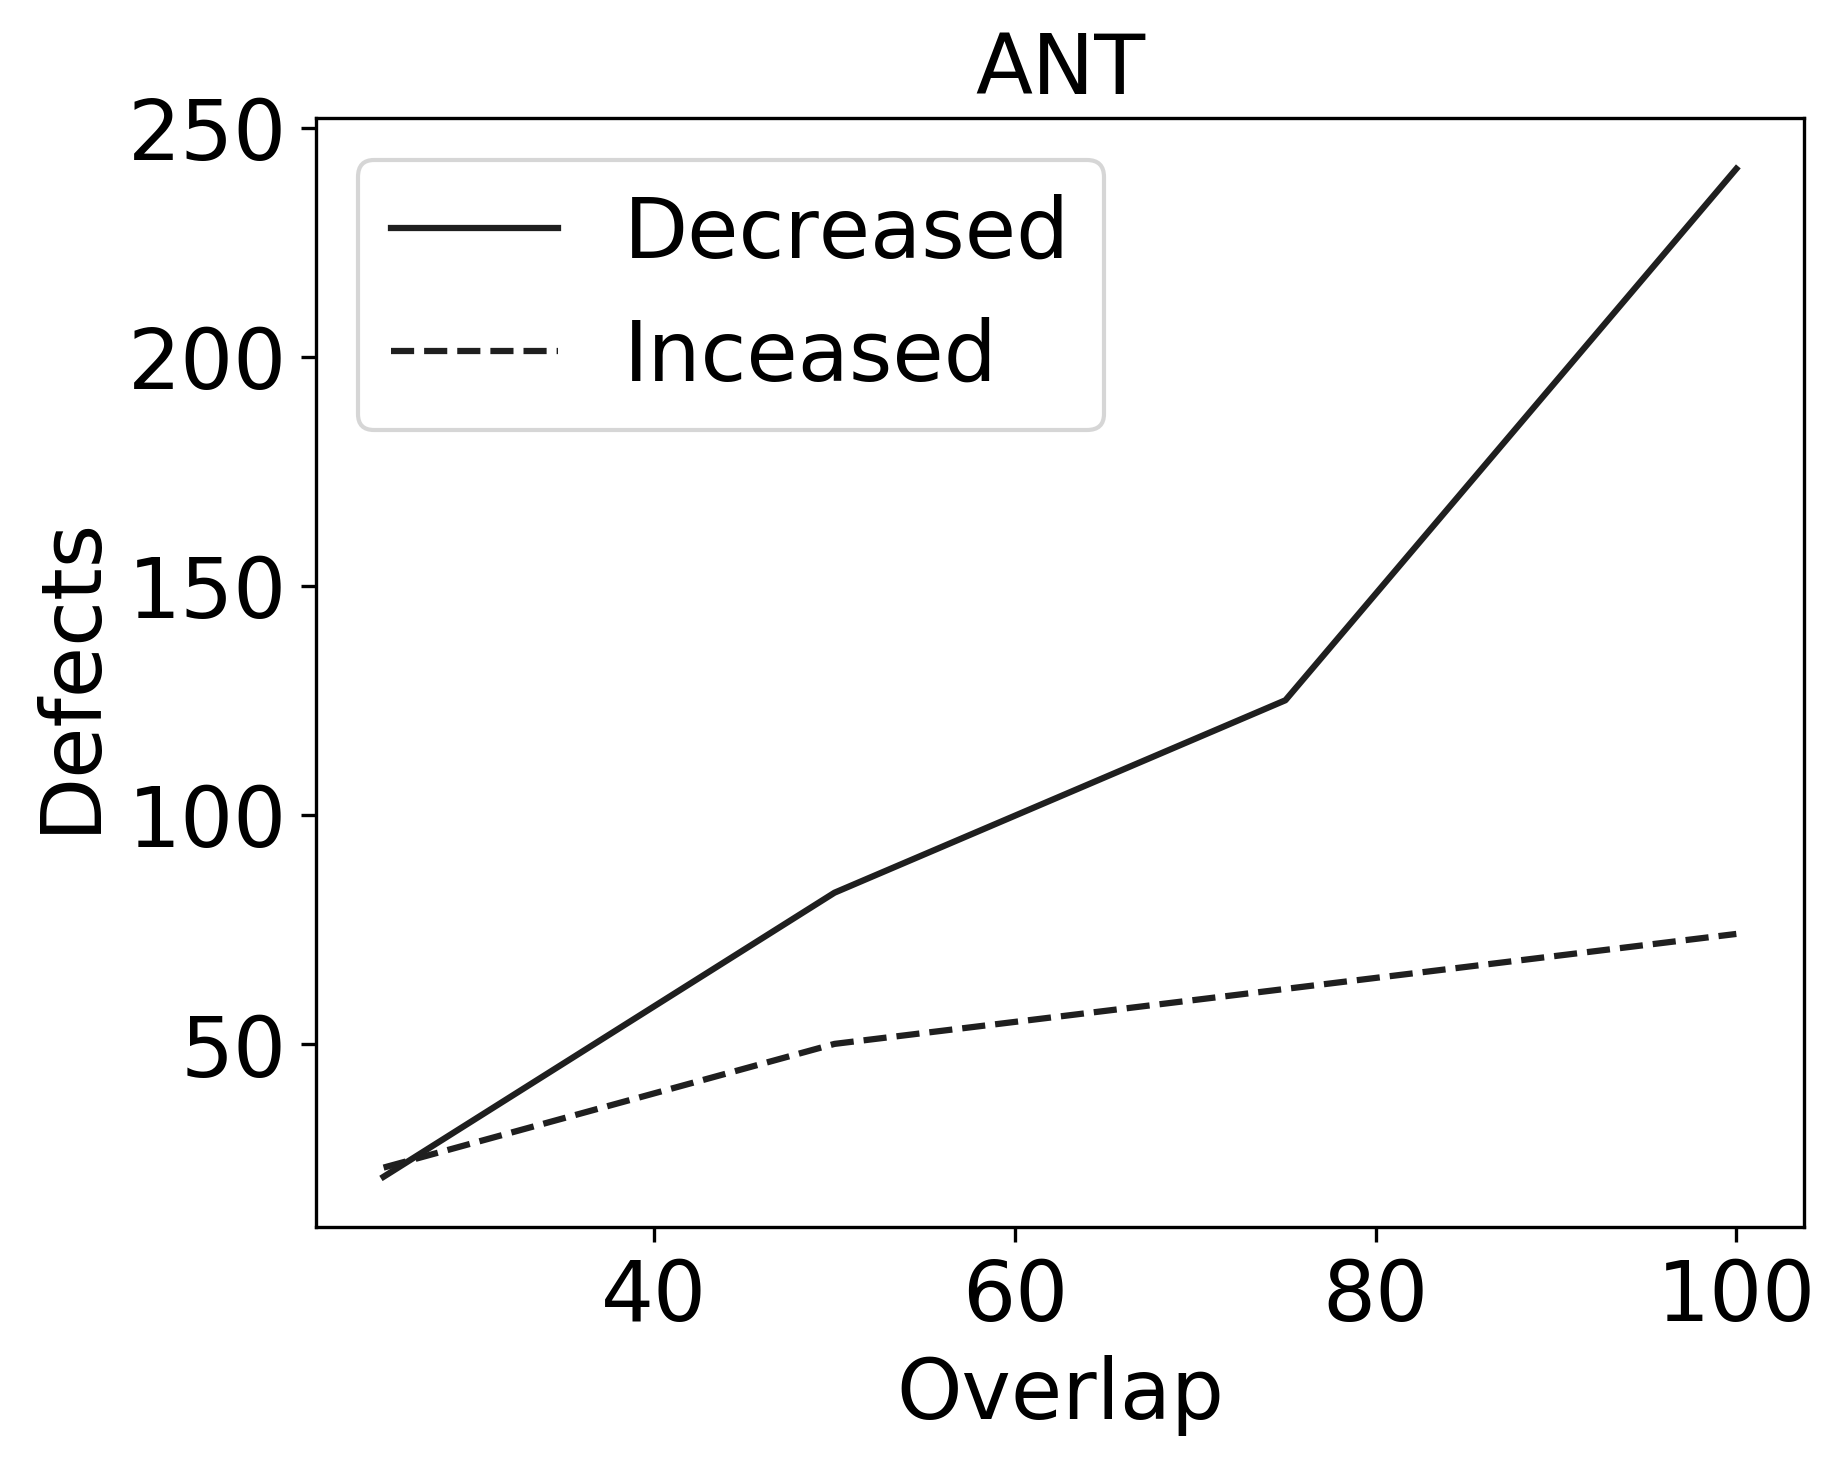
\includegraphics[width=0.7\linewidth]{images/sample_ant.png}
\end{center}
\[
\mathit{AUPEC} = \int_{0}^{1} f(x) \, dx \hfill
\]
\[\approx \tfrac{\Delta x}{3}\left(f(x_0) + 4f(x_1)+2f(x_2)+\cdots+4f(x_{n-1}) + f(x_{n})\right)
\]
Here, the variable $x$ represents the overlap between plans and developer changes
and  $f(x)$ represents the number of defects reduced as result of the overlap.\\

We should interpret AUPEC as follows:
\begin{enumerate}
    \item \textit{Defects Reduced:}
  AUPEC is always greater than zero and 
    \textit{larger values} of AUPEC point to \textit{more defects reduced} with increasing overlap.
    
        \item \textit{Defects Increased:}  AUPEC is still always greater than zero
        and \textit{smaller values} of AUPEC point to \textit{less defects increased} with increasing overlap.
   
\end{enumerate}
In the above plot, we show an example of XTREE on Ant. We see that the more developers used our plans (and moved right across the x-axis), then subsequent changes to the code removed far more defects than it added.  

Note: Since the actual number of defects vary from one project to another, we report the AUPEC score as a percentage of theoretical best. The theoretical best for AUPEC for defects reduced will be 100\% and 0\% for defects increased.
 
% On the other hand, in the right-hand-side figure,  when we look at defects \textit{increased}, XTREE still has a larger number of defects increased than other planners; but, the number of defects reduced in comparison to defects increased is significantly larger. Therefore, overall, we may assert that XTREE is a better planner.
\\\hline
\end{tabular}
\caption{ AUPEC = Area Under Planner Effectiveness Curve.}
\label{fig:report_sample}
\end{figure}

As the outcome of the \textit{k-test} we obtain the number of defects (increased or decreased) and the extent of overlap (from 0\% to 100\%). These enable us to plot the operating characteristic curve for the planners. The operating characteristic (OC) curve depicts the effectiveness of a planner with respect to the ability to reduce defects. The OC curve plots the overlap of developer changes with XTREE's recommendations versus the number of  defects reduced (referred to henceforth as planner effectiveness curve). A sample curve for one of our datasets in \fig{datasets} is shown in \fig{report_sample}.

For each of the datasets with versions $i, j, k$ we (1)~train the planner on version $i$; (2) deploy the planner to recommend plans for version $j$; and (3) validate plans for version $j$. Following this, we plot the planner effectiveness curve. Finally, we compute the area under the planner effectiveness curve (AUPEC) using the trapizoidal rule. See \fig{report_sample}
\begin{equation}
	\label{eq:diff}
	R=(1-\frac{\mathit{after}}{\mathit{before}})\times100\%
\end{equation}
The value of the measure $R$ has the following properties:
\bi
\item If $R = 0\%$, this means  ``no change from baseline''; 
\item If $R > 0\%$, this indicates ``improvement over the baseline'';
\item If $R < 0\%$, this indicates ``optimization failure''.
\ei


In addition to this, we count the frequency with which a certain code metric is changed. This is expressed as percentage change, measured using the following equation:
\begin{equation}
	\label{eq:change}
	\small
	Change=\frac{\mathit{\#times\ M\ changed}}{\mathit{\#test\ cases}}\times100\%~~~~\forall M \in OO\ Metrics
\end{equation}

\section{Planning in Software Analytics}
\label{sect:motivate}
\subsection{Implementing Planners}
\label{sect:planners}
In the previous sections, we introduced the notion of planning for decision making. In this section we offer a description of each of these planning methods:

\subsubsection{XTREE}
\label{sect:XTREE}


XTREE builds a decision tree,  then generates
plans by contrasting the differences between two branches:
(1)~the branch where you are; (2)~the branch to where you want to be.

XTREE takes a {\em supervised} $Cluster+Contrast$ approach to planning because we hypothesize that it is useful to reflect on the target class. Thus, XTREE uses a supervised decision tree algorithm of \fig{xtree}.A. To divide continuous numeric data, we use a Fayyad-Irani discretizer of \fig{xtree}.B.
Next, XTREE builds plans from the branches of the decision trees using the description of \fig{xtree}.C.
In doing so, we ask three questions, the last of which returns the plan:
\be
\item
Which {\em current} branch does a test case fall in?
\item Which {\em desired} branch would the test case want to move to?
\item What are the {\em deltas} between current and desired branches? 
\ee
These \textit{deltas} represent the threshold ranges\footnote{Thresholds are denoted by $[low,high)$ ranges for each metric} that represent the plans to reduce the defects. 


\subsubsection{BELLTREE}
BELLTREE is structurally similar to XTREE. It differs in the source of data used for analytics. While XTREE uses data from within the project, BELLTREE first starts by looking for the bellwether dataset. After finding the bellwether, BELLTREE constructs a decision tree to generate the plans.

To achieve this, we employ three operators -- DISCOVER, PLAN, VALIDATE:
    \be
    \item DISCOVER: {\em Check if the community has bellwether.} 
    This step is similar to our previous technique used to discover bellwethers~\cite{krishna16}. That is, we see if standard data miners can predict for the number of issues, given the static code attributes. This is done as follows:~ 
    \bi 
    \item
    For a community $C$ obtain all pairs of data from
    projects such that $P_i, P_j \in C$;
    \item
    Predict for defects in $P_j$ using a quality predictor learned from data taken from $P_i$;
    \item
    Report a bellwether if one $P_i$  generates consistently high predictions in a majority of $P_j \in C$.
    \ei
    \item PLAN: {\em Using the bellwether, generate plans to improve a new project data.} That is,
    having learned the bellwether on past data, we now construct a decision tree similar to XTREE. We use the same methodology to generate these plans.
    \item VALIDATE: {\em Go back  to step 1 if the performance statistics seen during PLAN fail to generate useful actions}.
    \ee
   Note the simplicity of this approach -- just wrap a for-loop around some data miners to discover the bellwether. Given the ubiquity of bellwethers~\cite{krishna17b}, this stage identifies bellwethers for each of the dataset studied here. These bellwethers are shaded in \colorbox{lavenderpink}{light gray} in~\fig{datasets}. 

Further, note that the use of bellwethers enables BELLTREE to leverage data from across different projects within a community. This presents a novel extension to XTREE which is limited to the used of data only from within a project.

% \subsubsection{BELLTREE}

% Much of software data analytics when it comes to tasks such as defect prediction, effort estimation, software refactoring, etc. revolve around two key questions: (a) which data (or metrics) are best suited to support a specific task, and (b) what can be learned by reasoning across the data. Given the availability of process and product data, the key task is to derive reusable lessons from this data. This task implicitly relates to the applicability of the data in real life practice. Software data for domains such as defect prediction is now widely available~\footnote{https://zenodo.org/}. As a result, defect prediction has seen constant and wide spread used of these data analytics. Hall et al. offers an extensive review on the   defect prediction literature~\cite{Hall2011}. Lessmann et al.~\cite{lessmann08} performed an extensive experimental comparison of different learning algorithms for defect prediction. Most defect predictors learned from static code attributes. Given software described in the attributes of \fig{static_metrics}, data miners can learn where the probability of software defects is highest. 



% In the area of software defect prediction, there are several contradictory findings. A classic example of such contradiction is the study by Zimmermann et al.~\cite{zimm}. They trained defect predictors on 622 pairs of projects and found that in only 4 percent of the pairs did the defect predictor learned from one project in a pair work on the other. This contradiction can be found also in using defect predictors constructed using OO metrics. While several researchers endorse the use of software metrics~\cite{halstead77,mccabe76, hall2000, chapman02, nagappan05}, several others~\cite{fenton00, shepperd94} are opposed to it. Menzies et al. highlighted 28 different studies that offered contradictory conclusion regarding several OO metrics. Their survey offered a troubling prospect to any practitioner hoping to draw inference about software metrics. Each study in this figure tend to indicate a clear preference for merit of a specific coding standard. But these preference differ from one study to another. For example, consider the depth of inheritance tree metric: in 11 out of 28 cases, studies indicate that this metric has a significant impact on defects, but in 14 cases conclusions are that this metric is not relevant. In fact, only response for class (rfc) seems to have a clear preference in all the studies. Menzies et al. reason that this instability is due the varied nature of the datasets and generally this points to a \textit{dataset drift} issue~\cite{localvsglobal,turhan_drift}. 

% The issue of data drift is only one source of instability. Menzies and Sheppard in their 2012 paper review several other sources of conclusion instabilities. These instabilities are broadly attributed to two major contributors: (a) bias and (b) variance. These result due a number of other causes as surveyed by Menzies and Sheppard~\cite{12instability}. They caution that their survey only highlights a partial list of causes that lead to instability which may serve as an inspiration to the research community to tame them.

% Such conclusion  instability is an unsettling prospect for practitioners. Software
% project managers find it increasingly difficult to generate general policies that can 
% offer clear insights into a number of issues including (a)~when a certain module should be inspected;
% (b)~when modules should  be refactored; (c)~where to focus
% expensive testing procedures; (d)~what return-on-investment
% might we expect due to decreased defects after purchasing an
% expensive tool; etc.

% To support those managers, who seek stability
% in their conclusions, while also allowing new projects
% to take full benefit from data arriving
% from all the other projects constantly
% being completed by other programmers is a difficult task. When it is not possible to {\em generalize} findings
% from all data, it is wise to seek a more achievable goal -- to {\em
% stabilize} the pace of conclusion change.
% While it may not be practical to wait for eternal and global SE
% conclusions, one possible approach is for organizations
% to seek methods that can offer analytics that can generalize across several projects over consistent periods of time. 

% One such method is the use of bellwether as proposed in our previous work~\cite{krishna16,krishna17b}.
% Our results showed that regardless of the sub-domain of software engineering (code smells, effort, defects or issue lifetimes) or granularity of data (see the file, class, file values of \fig{datasets}), there existed a bellwether data set that can be used to train relatively more accurate quality prediction models and this bellwether does not require elaborate data mining methods to discover (just a for-loop around the data 
% sets) and can be found very early in a project's life cycle (after analyzing only a few dozen  code modules). The stability offered by bellwethers can be leveraged to address the constant influx of new data that destabilizes conventional global models. 

% \section{Cross-project Planning}
% \label{sect:cross-planning}

% Much of the previous work on planning has assumed that the data for planning arises from the same project source. However, in several realistic scenarios, this is not a reasonable assumption. This issue has been addressed in defect prediction with the use of cross-project defect prediction. This issue of lack of local data persists when planning just as it did during prediction. Thus, a novel extension presented in this work is the idea of \textit{cross-project planning}. That is, using data from a different project to generate plans to improve the current project.

% We derived motivation for this from transfer learning from cross-project settings. Transfer Learning can be used to transfer lessons learned from other {\em source} projects $S$ to the {\em target} project $T$. A category of transfer learners called the \textit{homogeneous transfer learners} operate on datasets that share the same attributes. 

% Several studies over the past decade have shown the success of transfer learning in defect prediction. An initial attempt to perform transfer learning was undertaken by the Turhan et al~\cite{turhan09}. They introduced the \textit{Burak filter} which builds its
% training sets by finding the $k=10$ nearest code
% modules in $S$ for every $t\in T$. In other work, Ma et al.~\cite{Ma2012} with an algorithm called 
% transfer naive Bayes (TNB). This algorithm used information from all of the 
% suitable attributes in the training data. Based on the estimated distribution 
% of the target data, this method transferred the source information to 
% weight instances the training data. The defect prediction model was constructed using 
% these weighted training data. Nam et al.~\cite{Nam13} originally proposed an
% transform-based method that used TCA based
% dimensionality rotation, 
% expansion, and contraction to align the source
% dimensions to the
% target. They also proposed a new approach called TCA+, which selected suitable 
% normalization options for TCA.  However, the above transfer learning methods all suffer from
% the all too common instability problem described in the
% previous sections. Specifically, whenever the source or target is updated, data miners will learn a new  model every time.

% More recently, in ASE '16 Krishna et al.~\cite{krishna16} showed that a very simplistic transfer learner can be 
% developed using the ``bellwether" dataset with Random Forest. They reported highly competitive performance scores with this data and also showed that these datasets are stable sources for transfer learning.

% So far transfer learning has been used \textit{exclusively for prediction} tasks. However, the general premise of this technique allows for us to extend it to other tasks such as decision making. In this paper, we extend the notion of transfer learning and the ``bellwether'' dataset to decision making. We attempt to leverage these datasets to act as \textit{plan generators}. That is, we use this ``bellwether'' datasets to obtain very specific plans to improve the defect counts of projects within a community. We first use the \textit{bellwether method} to discover these bellwether datasets and use them exclusively for generating plans. Our reason for using bellwethers are as follows:
% \be
% \item These bellwethers are stable sources for planning. i.e., as long as the predictions of bellwethers remain the same, the lessons learned from it can be applied to the rest of the community. 
% \item They can be found very early in a project's life cycle (after analyzing 
% only a few dozen  code modules)
% \item They are also very prevalent. Although we discuss on defect prediction in this paper, bellwethers were shown to exist in several sub-domains in software engineering ranging from detection of code smells to prediction of issue lifetimes~\cite{krishna17b}. 
% \ee

% Therefore, instead of using other complex transfer learners to transfer plans from different projects and risk instability, we use bellwethers. 


\subsubsection{Alves}

Alves et al.~\cite{alves} proposed an unsupervised approach
that  uses the underlying statistical 
distribution and scale of the OO metrics. It works by first weighting each metric value according to the source lines of 
code (SLOC) of the class it belongs to. All the weighted metrics are then normalized by the sum of all weights for the system. The normalized metric values are ordered in an ascending fashion (this is 
equivalent to computing a density function, in which the x-axis represents 
the weight ratio (0-100\%), and the y-axis the metric scale).

Alves et al. then select a percentage value (they suggest 70\%) which 
represents the ``normal'' values for metrics. The metric threshold, then, 
is the metric value for which 70\% of the classes fall below. The 
intuition  is that the worst code has outliers beyond 70\% of the normal 
code measurements i.e., they state that the risk of there existing a defect 
is moderate to high when the threshold value of 70\% is exceeded.

Here, we explore the correlation between the code metrics 
and the defect counts with a univariate logistic regression and  reject 
code metrics that are poor predictors of defects (i.e.   those  with $p > 
0.05$). For the remaining metrics, we obtain the threshold ranges which are denoted by $[0,70\%)$ ranges for each metric. The plans would then involve reducing these metric range to lie within the thresholds discovered above.

\subsubsection{Shatnawi}

Shatnawi~\cite{shatnawi} offers a different alternative Alves et al by using VARL (Value of Acceptable Risk Level). This method was 
initially proposed by Bender~\cite{bender99} for his epidemiology studies.  This approach uses two
constants ($p_0$ and $p_1$) to compute the thresholds which Shatnawi recommends to be set to
$p_0=p_1=0.05$. 
Then using a univariate binary logistic regression three 
coefficients are learned:
$\alpha$ the intercept constant;
$\beta$ the coefficient for maximizing log-likelihood;
and $p_0$ to 
measure how well this  model predicts for defects. (Note: the univariate 
logistic regression was conducted comparing metrics to defect counts. Any 
code metric with $p>0.05$ is ignored as being a poor defect predictor.)

Thresholds are learned from the surviving metrics  using
the risk equation proposed by Bender:
$$ \mathit{Defective\ if}\ Metric > VARL$$
Where,
\begin{equation*}
	VARL = p^{-1}(p_0) =  \frac{1}{\beta }\left( {\log \left( 
		{\frac{{{p_1}}}{{1 - {p_1}}}} \right) - \alpha } \right)
\end{equation*}

In a similar fashion to Alves et al., we deduce the threshold ranges as $[0, VARL)$ for each selected metric. The plans would again involve reducing these metric range to lie within the thresholds discovered above.

\subsubsection{Oliveira}
Oliveira et al. in their 2014 paper offer yet another alternative to absolute threshold methods discussed above~\cite{oliveira}. Their method is still unsupervised, but they propose complementing the threshold by a second piece of information called the \textit{relative threshold}. This measure denotes the percentage of entities the upper limit should be applied to. These have the following format:
\begin{equation*}
	p\%\ of\ the\ entities\ must\ have\ M\leq k
\end{equation*}

Here, $M$ is an OO metric, $k$ is the upper limit of the metric value, and $p$ (expressed as \%) is the minimum percentage of entities are required to follow this upper limit. As an example Oliveira et al. state, `` $\ldots$ 85\% of the methods should have $CC \leq 14$. Essentially, this threshold expresses that high-risk methods may impact the quality of a system when they represent more than 15\% of the whole population of methods $\ldots$''

The procedure attempts derive these values of $(p,k)$ for each metric $M$. They define a function \texttt{ComplianceRate(p,k)} that returns the percentage of system that follows the rule defined by the relative threshold pair $(p,k)$. They then define two penalty functions: (1) \texttt{penalty1(p,k)} that penalizes if the compliance rate is less than a constant $Min\%$, and (2) \texttt{penalty2(k)} to define the distance between $k$ and the median of preset $Tail$-th percentile. (Note: according to Oliveira et al., median of the tail is an idealized upper value for the metric, i.e., a value representing classes that, although present in most systems, have very high values of M). They then compute the total penalty as \texttt{penalty} = \texttt{penalty1(p,k)} + \texttt{penalty2(k)}. Finally, the relative threshold is identified as the pair of values $(p,k)$ that has the lowest total \texttt{penalty}. After obtaining the $(p,k)$ for each OO metric. As in the above two methods, the plan would involve ensuring the for every metric $M$ $p\%$ of the entities have a value that lies between $(0,k]$\footnote{If certain metrics already satisfy this criterion, they remain unchanged}. 

\begin{figure}[tp!]
\centering
\resizebox{\linewidth}{!}{
\label{my-label}
\begin{tabular}{c|l|l|l|c|l|c}
& & \multicolumn{3}{c|}{Metrics} & \multicolumn{2}{c}{Class} \\ \hline
Version                & \multicolumn{1}{c|}{Module Name}                             & wmc                    & dit                    & \ldots & nDefects & isDefective \\ \hline
1.3                    & taskdefs.ExecuteOn & 11                     & 4                      & \ldots & 0        & FALSE       \\ \hline
1.3                    & DefaultLogger      & 14                     & 1                      & \ldots & 2        & TRUE        \\ \hline
\multicolumn{1}{c|}{\ldots} & \multicolumn{1}{c|}{\ldots}                  & \multicolumn{1}{c|}{\ldots} & \multicolumn{1}{c|}{\ldots} & \ldots & 0        & FALSE       \\ \hline
1.3                    & taskdefs.Cvs       & 12                     & 3                      & \ldots & 0        & FALSE       \\ \hline
1.3                    & taskdefs.Copyfile  & 6                      & 3                      & \ldots & 1        & TRUE       
\end{tabular}}
\caption{A sample of ant 1.3}
\label{fig:example}
\end{figure}

\begin{figure*}[htbp]
\centering
\captionsetup[subfigure]{width=\linewidth}
\subfloat[][Plans recommended by XTREE]{
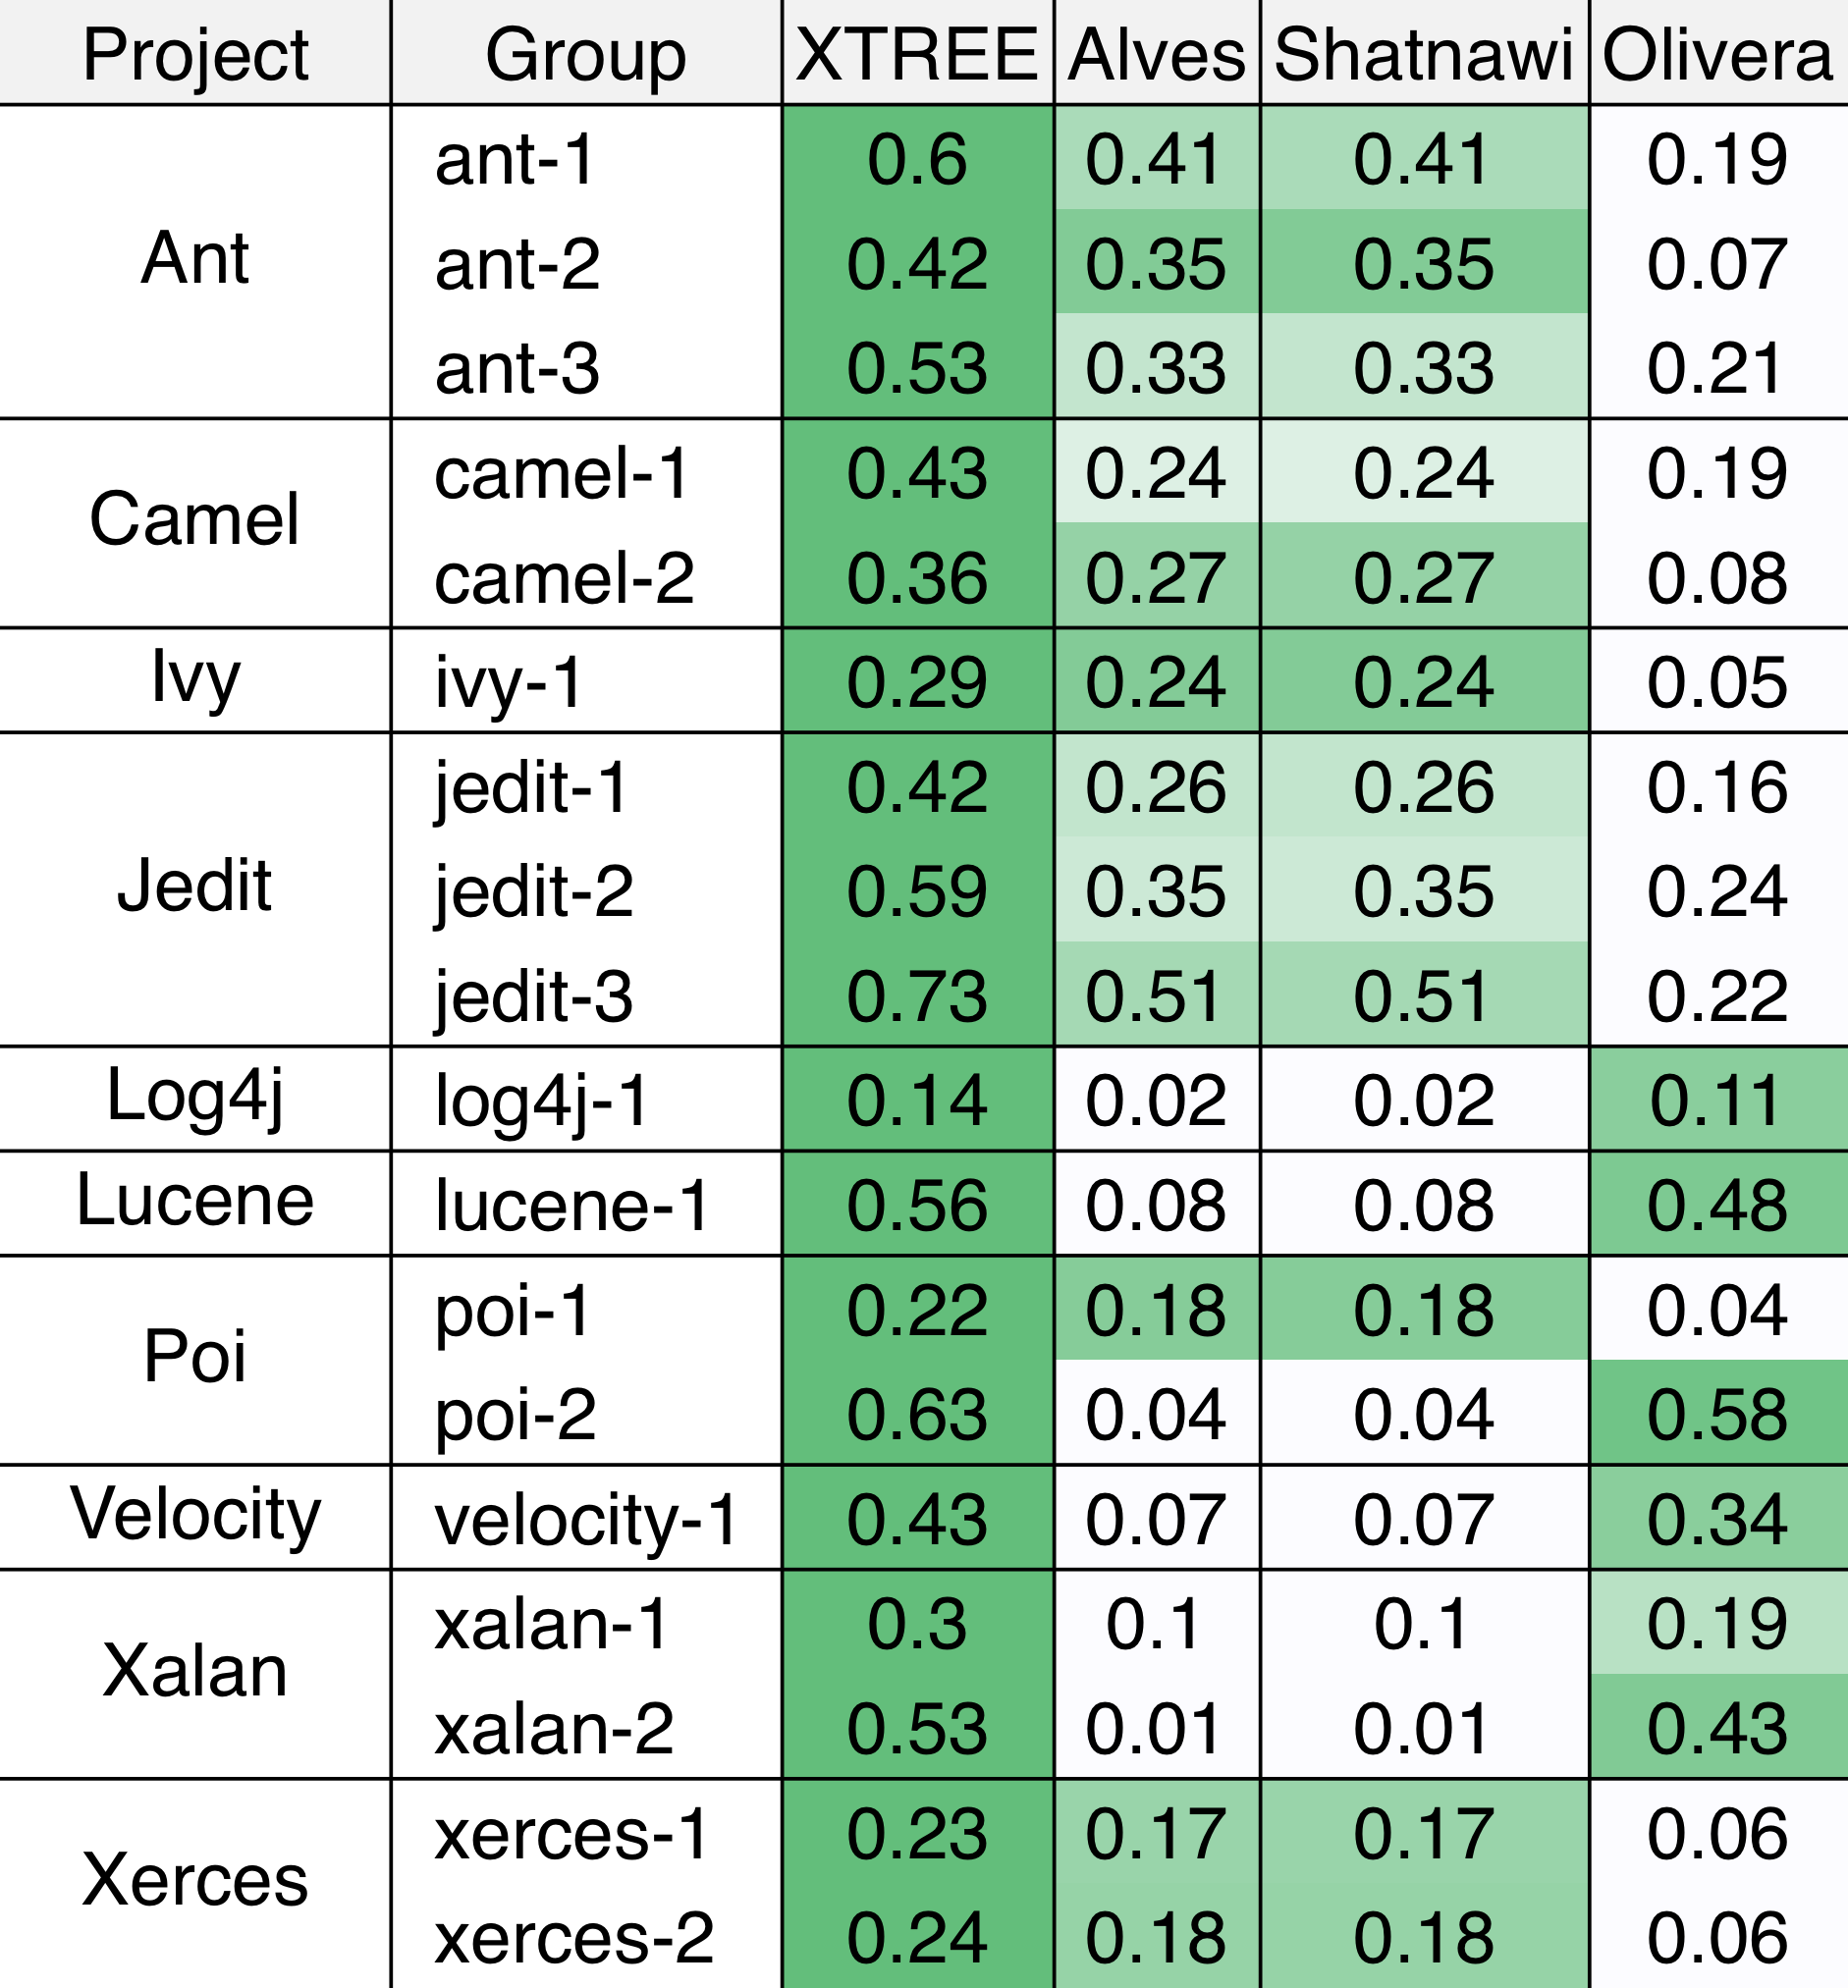
\includegraphics[width=0.4\linewidth]{images/RQ3/RQ3.png}}
\qquad\qquad
\subfloat[][Plans recommended by XTREE]{
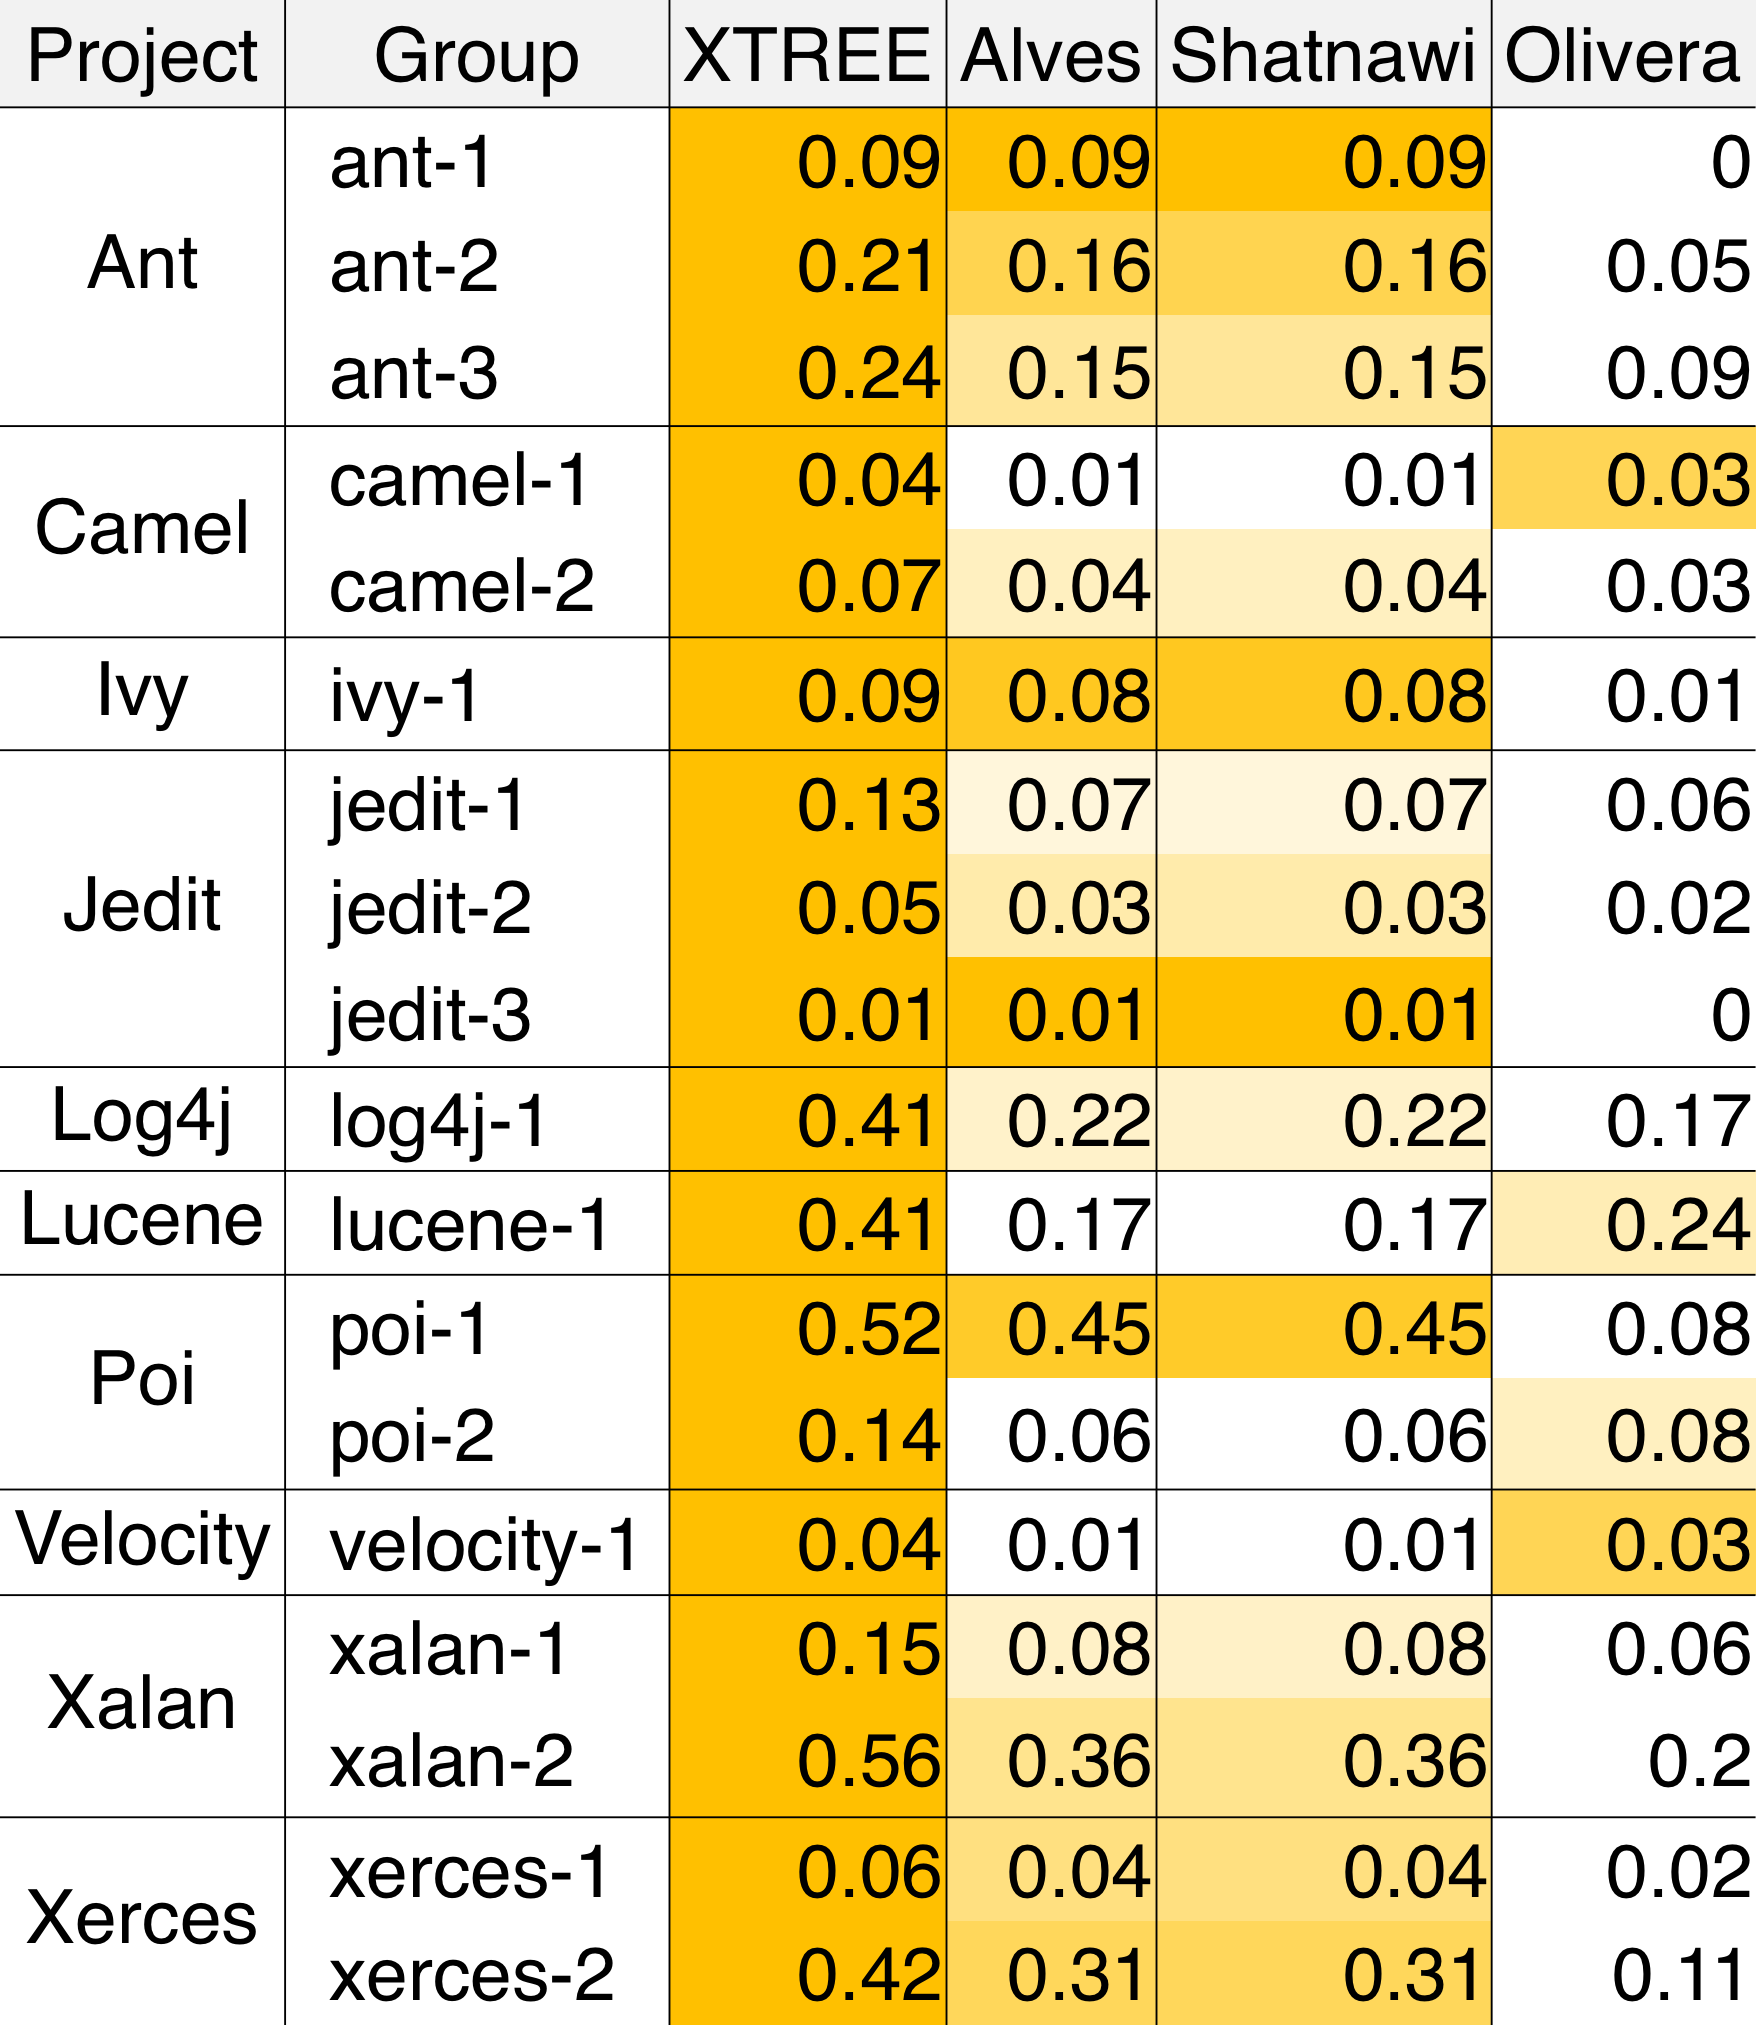
\includegraphics[width=0.375\linewidth]{images/RQ3/RQ3_2.png}}
\caption{This figure shows forecasts for future bugs and enhancements using ARIMA models constructed using past issue reports. For both proprietary and opensource projects, the magnitude of average error is very low (close to zero in several cases). Trend graphs show that an increase in actual bugs (or enhancements) leads to a corresponding increase in forecasts.}
\label{fig:rq3}
\end{figure*}

\begin{figure*}[ht!]
\renewcommand{\baselinestretch}{0.7}
  \centering
  \begin{minipage}{\linewidth}
  \resizebox{\linewidth}{!}{
    \begin{tabular}{l@{~}|r@{~}r|@{~}r@{~}r@{~}r|r@{~}r|r@{~}r@{~}r|r@{~}r|r@{~}r@{~}r|r@{~}r|r@{~}r@{~}r}
          & \multicolumn{5}{c|}{Ant}              & \multicolumn{5}{c|}{Jedit}            & \multicolumn{5}{c|}{Ivy}              & \multicolumn{5}{c}{Poi} \bigstrut\\
\cline{2-21}          & \multicolumn{2}{c|}{$Cluster+Contrast$} & \multicolumn{3}{c|}{Statistical Thresholding} & \multicolumn{2}{c|}{$Cluster+Contrast$} & \multicolumn{3}{c|}{Statistical Thresholding} & \multicolumn{2}{c|}{$Cluster+Contrast$} & \multicolumn{3}{c|}{Statistical Thresholding} & \multicolumn{2}{c|}{$Cluster+Contrast$} & \multicolumn{3}{c}{Statistical Thresholding} \bigstrut\\
          & \multicolumn{1}{l}{BELLTREE} & \multicolumn{1}{l|}{XTREE} & \multicolumn{1}{l}{Oliveira} & \multicolumn{1}{l}{Alves} & \multicolumn{1}{l|}{Shatnawi} & \multicolumn{1}{l}{BELLTREE} & \multicolumn{1}{l|}{XTREE} & \multicolumn{1}{l}{Oliveira} & \multicolumn{1}{l}{Alves} & \multicolumn{1}{l|}{Shatnawi} & \multicolumn{1}{l}{BELLTREE} & \multicolumn{1}{l|}{XTREE} & \multicolumn{1}{l}{Oliveira} & \multicolumn{1}{l}{Alves} & \multicolumn{1}{l|}{Shatnawi} & \multicolumn{1}{l}{BELLTREE} & \multicolumn{1}{l|}{XTREE} & \multicolumn{1}{l}{Oliveira} & \multicolumn{1}{l}{Alves} & \multicolumn{1}{l}{Shatnawi} \bigstrut\\\hline
    
    rfc   & 100   & 100   & 42    & 62    & 50    & 100   & 100   & 50    & 45    & 100   & $\cdot$     & 53    & 46    & 60    & 50    & 100   & 50    & 8     & 14    & 100 \bigstrut\\
    lcom  & $\cdot$     & $\cdot$     & 32    & 70    & 100   & $\cdot$     & $\cdot$     & 40    & 54    & 100   & $\cdot$     & $\cdot$     & 35    & 76    & 100   & $\cdot$     & $\cdot$     & 15    & 69    & 100 \bigstrut\\
    cam   & $\cdot$     & 46    & $\cdot$     & 23    & 100   & $\cdot$     & $\cdot$     & $\cdot$     & 63    & 100   & 100   & $\cdot$     & $\cdot$     & 52    & 100   & $\cdot$     & $\cdot$     & $\cdot$     & 64    & 100 \bigstrut\\
    ce    & $\cdot$     & $\cdot$     & 17    & 47    & 100   & $\cdot$     & $\cdot$     & 40    & 54    & 100   & 1     & 53    & 27    & 31    & 100   & $\cdot$     & $\cdot$     & 5     & 42    & 100 \bigstrut\\
    mfa   & $\cdot$     & 46    & 8     & 40    & 100   & $\cdot$     & $\cdot$     & 27    & 45    & 100   & 32    & $\cdot$     & $\cdot$     & 20    & 100   & $\cdot$     & $\cdot$     & 2     & 50    & 100 \bigstrut\\
    amc   & $\cdot$     & 46    & 4     & 17    & 100   & $\cdot$     & 50    & $\cdot$     & $\cdot$     & 100   & 22    & 50    & 11    & 3     & 100   & $\cdot$     & 50    & 3     & 8     & 100 \bigstrut\\
    dit   & $\cdot$     & $\cdot$     & 23    & 41    & 100   & $\cdot$     & $\cdot$     & 40    & 45    & 100   & $\cdot$     & $\cdot$     & 16    & 17    & 100   & $\cdot$     & $\cdot$     & $\cdot$     & 50    & 100 \bigstrut\\
    cbo   & 50    & 50    & 9     & 14    & 43    & $\cdot$     & 50    & 27    & 54    & 40    & $\cdot$     & 46    & 25    & 53    & 48    & $\cdot$     & 99    & 4     & 5     & 13 \bigstrut\\
    ca    & $\cdot$     & $\cdot$     & 4     & 13    & 100   & $\cdot$     & 50    & 18    & 50    & 100   & 1     & 50    & 11    & 18    & 100   & $\cdot$     & $\cdot$     & 3     & 3     & 100 \bigstrut\\
    max cc & $\cdot$     & $\cdot$     & 23    & 46    & 100   & $\cdot$     & $\cdot$     & 18    & 59    & 100   & $\cdot$     & $\cdot$     & 13    & 35    & 100   & $\cdot$     & $\cdot$     & 5     & 14    & 100 \bigstrut\\
    avg cc & $\cdot$     & $\cdot$     & 14    & 56    & 100   & $\cdot$     & $\cdot$     & 13    & 31    & 100   & 50    & $\cdot$     & 6     & 27    & 100   & $\cdot$     & $\cdot$     & 4     & 8     & 100 \bigstrut\\
    npm   & $\cdot$     & $\cdot$     & 24    & 38    & 53    & $\cdot$     & $\cdot$     & 31    & 36    & 50    & 27    & $\cdot$     & 41    & 52    & 50    & $\cdot$     & 49    & 25    & 24    & 100 \bigstrut\\
    loc   & $\cdot$     & 46    & 22    & 43    & 10    & $\cdot$     & $\cdot$     & 22    & 54    & 13    & 51    & 96    & 27    & 48    & 18    & 99    & $\cdot$     & 5     & 17    & 3 \bigstrut\\
    ic    & $\cdot$     & $\cdot$     & 9     & 18    & 100   & $\cdot$     & $\cdot$     & 13    & 18    & 100   & $\cdot$     & $\cdot$     & 2     & 18    & 100   & $\cdot$     & $\cdot$     & $\cdot$     & 34    & 100 \bigstrut\\
    wmc   & $\cdot$     & $\cdot$     & 30    & 43    & 61    & $\cdot$     & $\cdot$     & 36    & 40    & 68    & $\cdot$     & $\cdot$     & 35    & 50    & 50    & $\cdot$     & $\cdot$     & 17    & 23    & 50 \bigstrut\\
    dam   & $\cdot$     & $\cdot$     & $\cdot$     & $\cdot$     & 100   & $\cdot$     & $\cdot$     & $\cdot$     & 18    & 50    & $\cdot$     & $\cdot$     & $\cdot$     & 31    & 100   & $\cdot$     & $\cdot$     & $\cdot$     & 47    & 100 \bigstrut\\
    noc   & $\cdot$     & $\cdot$     & 5     & 15    & 100   & $\cdot$     & $\cdot$     & $\cdot$     & $\cdot$     & 100   & $\cdot$     & $\cdot$     & 3     & 5     & 100   & $\cdot$     & $\cdot$     & 3     & 6     & 100 \bigstrut\\
    moa   & $\cdot$     & $\cdot$     & 8     & 35    & 51    & $\cdot$     & $\cdot$     & 36    & 45    & 100   & $\cdot$     & $\cdot$     & 11    & 30    & 57    & $\cdot$     & $\cdot$     & 6     & 17    & $\cdot$ \bigstrut\\
    cbm   & $\cdot$     & $\cdot$     & 16    & 12    & 50    & $\cdot$     & $\cdot$     & 13    & 18    & 50    & $\cdot$     & $\cdot$     & 6     & 20    & 50    & $\cdot$     & $\cdot$     & 49    & 55    & 50 \bigstrut\\
    lcom3 & $\cdot$     & 3     & $\cdot$     & 21    & $\cdot$     & $\cdot$     & $\cdot$     & $\cdot$     & 63    & $\cdot$     & 27    & $\cdot$     & $\cdot$     & 66    & $\cdot$     & $\cdot$     & $\cdot$     & $\cdot$     & 45    & $\cdot$ \bigstrut\\
    \hline
    \end{tabular}}%
\end{minipage}
\caption{Results for {\bf RQ5}.
Percentage counts of  how often each planner recommends changing a code metric
(in 40 runs). ``100'' means that this code metric
was always recommended. Cells marked with ``.'' indicate  0\%. For the Shatnawi, Alves et al., and Oliveira et al.
columns,  metrics score 0\% if they always fail the p $\le$ 0.05 test proposed by shatnawi in \tion{planners}. Note
that textit{Cluster+Contrast} mentions specific code metrics
far fewer times than other methods.}
  \label{fig:rq2_1}%
\end{figure*}%




\section{Experimental Results}
\label{sect:results}

\subsection*{{\bf RQ1: Does within project planning offer statistically significant results?}}

To answer this question, we first identify the sources of data: i.e., data local to a specific project. Next, with these these sources of data we construct models for planning using the methods described in \tion{planners}. 

Next, using a separate data, that was not used in planning, we construct a verification oracle to study the \textit{impact} of these plans.  If planning were to have a significant response to defect reduction, we would ideally like to have $R>0\%$. In a result consistent with previous reports by Krishna et al.~\cite{krishna17a}, we find that all methods have a positive impact on defect reduction.

\fig{rq1} shows the results of planning with various planners discussed in \tion{planners}. These figure tabulate the percent improvements in defects defined by \eq{diff}. We note that, all the planners result in improvements greater than 0\% which means that all these planners have a positive impact on reducing the number of defects.

We note that some planners were better than others in reducing defect counts. This is discussed in RQ2. To summarize, for a post-hoc planning, both supervised planners like XTREE and unsupervised methods of Alves, Shatnawi, Oliveria are capable of offering positive and statistically significant improvements. Therefore, we answer \textbf{RQ1} as follows:

%\begin{lesson}
%	Within project planning offers statistically significant improvement while 
%planning.\\[-.2cm]
%\end{lesson}

\subsection*{{\bf RQ2: Does using XTREE for within project planning offer benefits over other unsupervised methods?}}

To answer this question, we first identify the sources of data: i.e., data local to a specific project, as in RQ1. Next, with these sources of data we construct models for planning using the methods described in \tion{planners}. Using a verification oracle, we  compare the Scott-Knott results of each of the supervised and unsupervised planners. 

\fig{rq1} shows that in 6 of 8 test datasets, XTREE offers statistically better performance compared to other unsupervised methods. In the Jureczko community of datasets, we note that learning plans from XTREE data has much lower IQR than other planners. We attribute this to the unsupervised nature of the other planners. Specifically, these unsupervised planners use thresholds on metrics to indicate what needs to be changed. These thresholds always remain the same for a dataset and do not change with the test cases. As a result, large variances result from applying them. This, is also what sets XTREE apart from these planners. XTREE adapts the plans based on the test cases thereby resulting in better performance and lower variances. Hence:

%\begin{lesson}
%	With local data, plans derived from XTREE have significantly better 
%performance and much lower variance compared to other planners.\\[-.2cm]
%\end{lesson}

\begin{figure}[htbp]
\centering
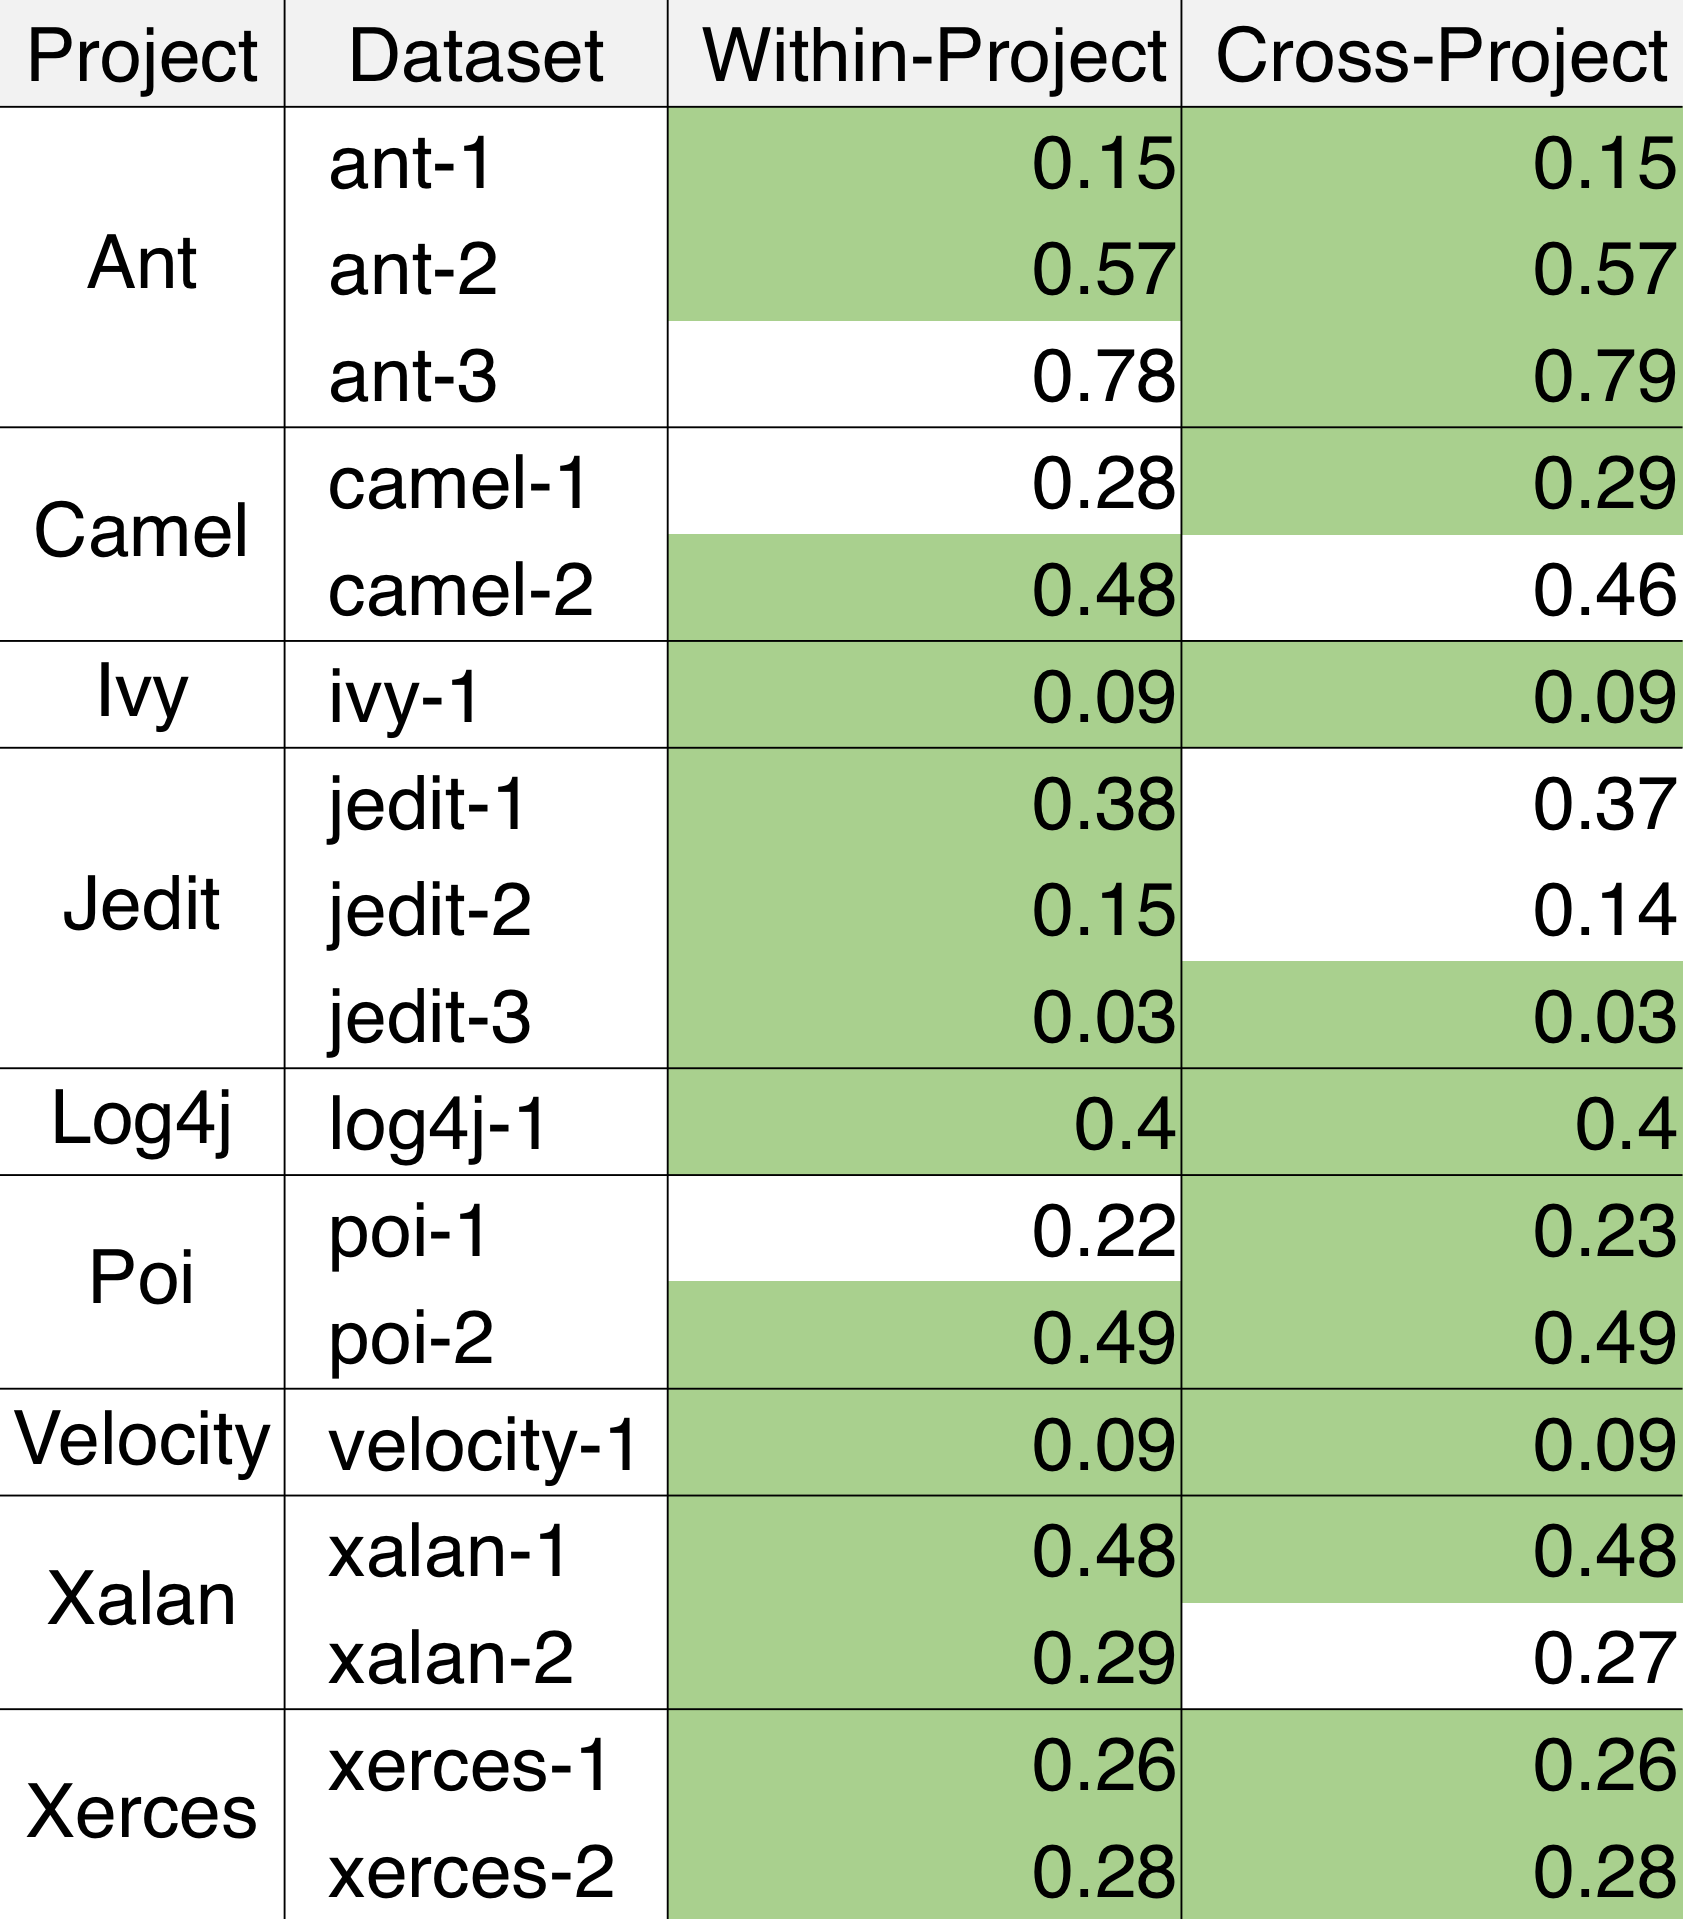
\includegraphics[width=0.75\linewidth]{images/RQ4_5/RQ4_5.png}
\caption{This figure shows forecasts for future bugs and enhancements using ARIMA models constructed using past issue reports. For both proprietary and opensource projects, the magnitude of average error is very low (close to zero in several cases). Trend graphs show that an increase in actual bugs (or enhancements) leads to a corresponding increase in forecasts.}
\label{fig:rq4_5}
\end{figure}


\subsection*{{\bf RQ3: How stable are the plans generated by XTREE as we move across different projects?}}

This question naturally arises from the outcomes of the previous research questions. There we noted that plans generated using XTREE produced significantly better improvements compared to other planners. Here, we ask if that is due to XTREE recommending a consistent set of plans for each dataset. To answer this, we aggregate the recommended plans for each dataset that used XTREE.  

Figure~\ref{fig:rq2_1} shows the frequency with which the source code metrics are recommended for change by the planners under study. The frequency of changes were measured using \eq{change}. We make the following observations with regards to XTREE with this: 
\be
\item XTREE propose changes to much fewer code metrics compared to the other unsupervised approaches. At the same time, as per \fig{rq1}, XTREE produce the overall best performance. 
\item More interestingly, XTREE recommends different plans for different datasets. Only certain metrics are changed in all the datasets, E.g., ~$rfc$ and $amc$ (in Jureczko datasets);
\ee

From the above, we note that it is not necessary to change multiple metrics to improve defects. Using different sources of data to train a planner, a similar result, that of reducing defects, can be achieved by changing different subsets of metrics. There is no single metric, that can be changed in all datasets to achieve consistently good performance. This is disconcerting, it is highly likely that these plans will change entirely when new training data arrives, or as dataset drifts over time. This leads to unstable conclusions.

Additionally, on further inspection of~\fig{rq2_1}, it can be noticed that unsupervised planners (Shatnawi, Alves, and Oliveira) recommend changing almost all of the code metrics. However, this is not a practical alternative, and may render much of these suggestions useless. Note that these unsupervised methods also suffer from ``conjunctive fallacy''. That is, they assume that the best way to reduce defects is to decrease multiple code metrics to lie below a threshold while not accounting for the intricate dependencies between the code metrics. We therefore deprecate these unsupervised planners in favor of supervised planners like XTREE. In conclusion, we answer \textbf{RQ3} as follows: 

%\begin{lesson}
%	XTREE recommends changing different metrics for different datasets. This 
%points to conclusion instability because arrival of new data would lead to 
%completely different plans.\\[-.2cm]
%\end{lesson}

\subsection*{{\bf RQ4: Does cross-project planning with BELLTREE offer statistically significant improvements compared to other methods?}}

In this research question, we compare the use of BELLTREE planner with other unsupervised planners. To answer this research question, we conduct experiments similar to RQ2. That is we, train the planners on bellwether data and generate plans for reducing the number of defects.

We then use Scott-Knott to statistically compare BELLTREE with other planners similar to the procedure in RQ2. We note that the use of BELLTREE offered statistically significant improvements compared to other methods.

\fig{rq1} shows the comparison between BELLTREE and other unsupervised planners. Note that, as with RQ2, BELLTREE outperforms other unsupervised planners. 

Further, in some planners such as Alves et al. using the bellwether data to generate plans in an unsupervised fashion results in increasing the number of defects instead of decreasing it (the R scores are negative). Additionally, as noted in \fig{rq2_1}, except for BELLTREE other planners recommend changes to almost all the metrics, most of the times, this cannot be considered a realistic approach as we discussed in RQ3. Thus, our answer to this research question is as follows:

%\begin{lesson}
%As with using local data sources, BELLTREE offers statistically significant 
%improvements over other planners.\\[-0.2cm]
%\end{lesson}

\subsection*{{\bf RQ5: Are BELLTREE's cross-project plans any better than XTREE's within project plans?}}

To answer this research question, we train the planners on within-project data and generate plans for reducing the number of defects. We then compare this with plans derived from the bellwether data for that community. We hypothesized that since bellwethers have been demonstrated to be efficient in prediction tasks, learning from the bellwethers for a specific community of projects would produce performance scores comparable to within-project data. We found that this was indeed the case; i.e. when viewed in terms of \textit{impact}, both XTREE and BELLTREE are similar.

\fig{rq1_1} tabulates the comparison between the use of XTREE and BELLTREE planning using the bellwether data set. The bellwethers for each community are highlighted in \fig{datasets}. We note that in 6 out of 8 datasets, both plans generated from the bellwether and the local datasets are ranked similarly by the scott-knott test. 

This finding has a major significance. The use of bellwether data implies that we use the same dataset to generate plans for all the project. As long as the bellwether data remains unchanged, so would the plans derived from it. This means that we can expect stable plans from BELLTREE. This is in contrast to
using XTREE, where plans may change over time leading to unstable conclusions.

In summary, we make the following observations:

%\begin{lesson}
%The performances of cross-project planning using BELLTREE and within project 
%planning using XTREE are similar. If within-project data is available, we 
%recommend using XTREE. If not, using bellwethers would be a reasonable 
%alternative.\\[-0.2cm]
%\end{lesson}

\section{Discussion}
\label{sect:discuss}
\subsection*{\textit{2. Why use automatic methods to find quality plans? Why not just use domain knowledge; e.g. human expert intuition?}}

Much recent work has documented the wide variety of conflicting
opinions among software developers, even those working within the same project. According to Passos et al.~\cite{passos11}, developers often assume that the lessons they learn from a few past projects are general to all their future projects. They comment, “past experiences were taken into account without
much consideration for their context” [34]. Jorgensen and Gruschke~\cite{jorgensen09} offer a similar warning. They report that the supposed software engineering ``gurus” rarely use lessons from past projects to improve their future reasoning and that such poor past advice can be detrimental to new projects~\cite{jorgensen09}. Other studies have shown some widely-held views are now questionable given new evidence. Devanbu et al. examined responses from 564 Microsoft software developers from around the world. They comment programmer beliefs can vary with
each project, but do not necessarily correspond with actual evidence
in that project~\cite{prem16}.

Given the diversity of opinions seen among humans, it seems wise to explore automatic oracles for planning quality improvement change.

\subsection*{\textit{3. Do bellwethers guarantee that software managers will never have to change their plans?}}

No. Software managers should evolve their policies when the evolving circumstances require such an update. But how to know when to retain currently policies or when to switch to new ones? Bellwether methods can answer this question.

Specifically, we advocate continually retesting the bellwether's status against other data sets within the community. If a new bellwether is found,
then it is time for the community to accept very different policies. Otherwise, it is valid for managers to ignore most the new data arriving into that community.

\section{Threats to Validity}
\label{sect:threats}
\subsection{Sampling Bias} 
Sampling bias threatens any classification experiment;
what matters in one case may or may not hold in another case. 
For example, even though we use a number of open-source datasets in 
this study which come from several sources, they were 
all supplied by individuals.  

That said, this paper addresses this sampling bias problem.  As researchers, all we can do is document
our selection procedure for data and suggest that other researchers
try a broader range of data in future work.



\subsection{Learner Bias} 
For building the verification oracle in this
study, we elected to use random forests. We chose this learner
because past studies shows that, for prediction tasks, the 
results were superior to other more complicated algorithms~\cite{lessmann08}  
and can act as a baseline for other algorithms. 

Apart from this choice,
one other limitation to our current study is that we have focused here
on one supervised planner (XTREE) and a number of unsupervised planners.
The implications of our findings are limited by the efficacy of the verification oracle. We understand the implication 
of this, and thus propose undertaking a preliminary study to validate the verification oracle. The rest of the analysis can be 
limited to those datasets where the learner has satisfactory performance.


\subsection{Evaluation Bias}
This paper uses one measure for the quality of prediction the oracle (Recall and False Alarm) and for the planners we use R (see Equation 1). 
Other quality measures often used in software engineering to quantify
the effectiveness of prediction~\cite{ma07}~\cite{Menzies2007a}~\cite{fu16}. A comprehensive analysis using these measures may be performed with our replication package. Additionally, other measures can easily be added to extend this replication package.

\subsection{Order Bias} 

With random forest and the planners, there is invariably some degree of randomness that is introduced by both the algorithms. Random Forest, as the name suggests, randomly samples the data and constructs trees which it then uses in an ensemble fashion to make predictions. 

To mitigate these biases, we run
the experiments 30 times (the reruns are equal to 30 in keeping with the central limit theorem). Note that the reported variations over those runs
were very small.
Hence, we conclude that while order bias is theoretically a problem,
it is not a major problem in the particular case of this study.

\section{Conclusions and Future Work}
\label{sect:future}
% It is quite evident that there is a rapid growth of the use of data analytics in software engineering. Such a growth has revealed some open issues that need to be tackled. This paper is an attempt to address these issues.  

Most software analytic tools that are currently in use today are mostly prediction algorithms. These algorithms are limited to making predictions. We extend this by offering ``planning'': a novel technology for prescriptive software analytics. Our planner offers users a guidance on what action to take in order to improve the quality of a software project. Our preferred planning tool is BELLTREE, which performs cross-project planning with encouraging results. With our BELLTREE planner, we show that it is possible to reduce defects in software projects by $>50\%$ in 6 out of 8 cases (note that in several cases, we achieved $>90\%$ reduction). 

It is also worth noting that BELLTREE is a novel extension of our prior work on (1) the bellwether effect, and (2) within-project planning with XTREE. With the bellwether effect we demonstrated that we can use stable sources of data to perform cross-project defect prediction without the need for more complex transfer learners. With XTREE we introduced a supervised $Cluster+Contrast$ planning framework that can be used to generate effective within-project plans. In this work, we show that it is possible to use bellwether effect and within-project planning (with  XTREE) to perform cross-project planning using BELLTREE. Our results from~\fig{rq1_1} show that in 4 out of 8 cases, BELLTREE is just as good as XTREE and in the remaining 4 cases XTREE performs only marginally better than BELLTREE.

Further, we can see from \fig{rq2_1} that both BELLTREE and XTREE recommend changes to very few metric, while other unsupervised planners such as Shatnawi, Alves, and Olivera, recommend changing most of the metrics. This is not practical in many real world scenarios.

Finally, we note that BELLTREE can offer stable solutions. As long as the bellwether data from which BELLTREE is constructed remains unchanged, so would plans that are derived from it. In this sense, practitioners can expect stable plans for relatively longer periods of time. This is in contrast to our XTREE planner. As more within-project data is gathered,  it is important that XTREE planner be updated. Such constant updates would invariably lead to unstable and often contradicting plans.


As for future work, we would like to undertake the following tasks:
\be
\item \textit{Industrial validation}: One of immediate goals is to validate the 
usefulness of these planners in a realistic development environment. As the 
first steps towards this, we are currently collaborating with a software 
company in RTP to deploy XTREE in their pipeline. 
\item \textit{Developer survey: }It would also be valuable to solicit 
developers' feedback on planners such as XTREE. A study of their willingness to 
use such tools would greatly benefit the software analytics community.
\item \textit{Scaling planners:} It must be noted that the datasets studied 
here are relatively small. In order to be able to use XTREE as a real time 
planner for very large projects. It is very important to scale these planners 
to accommodate very large datasets.
\ee

\balance
\bibliographystyle{IEEEtran}
\bibliography{References}

\end{document}